\documentclass{article}

\usepackage{times}

\usepackage{graphicx}

\usepackage{multirow}
\usepackage{amsmath}
\usepackage{amsthm}
\usepackage{amssymb,latexsym,color}
\usepackage{mdwlist}
\usepackage{todonotes}
%\usepackage{fullpage}
%\usepackage{charter}

\usepackage{url}

\usepackage{wrapfig}

%\usepackage{algorithm}
%\usepackage[noend]{algpseudocode}

%\usepackage{fullpage}
\usepackage{marvosym}
%\usepackage[techreport]{systems-cover}
\usepackage{natbib}
\usepackage{graphicx}
\graphicspath{ {Figures/} }
\usepackage{subcaption}
%\captionsetup[subfigure]{justification=justified,singlelinecheck=false}

\newcommand{\R}{\mathsf{R}}
\newcommand{\sgn}[1]{\mbox{sgn}(#1)}
\renewcommand{\vec}[1]{\mathbf{#1}}

\def\a{{\bf a}}
\def\g{{\bf g}}
\def\x{{\bf x}}
\def\y{{\bf y}}
\def\w{{\bf w}}
\def\v{{\bf v}}
\def\E{\mathbb{E}}
\def\rrow{r_\mathrm{row}}

\newcommand{\err}{\ensuremath{\mathrm{err}}}
\newcommand{\setX}{\Omega}
\newcommand{\setI}{\mathcal{I}}
\newcommand{\OPT}{\ensuremath{\mathrm{OPT}}}

\def\Ji{Ji's comment}

\DeclareMathOperator*{\argmin}{argmin}

\newtheorem{lemma}{Lemma}
\newtheorem{theorem}{Theorem}
\newtheorem{claim}{Claim}
\newtheorem{corollary}{Corollary}
\newtheorem{prop}{Proposition}
\newtheorem{definition}{Definition}

%\newcommand{\todo}[1]{\noindent \textbf{[TODO:] #1 } }
\usepackage{mathtools}
\DeclarePairedDelimiter\floor{\lfloor}{\rfloor}
\DeclarePairedDelimiter\ceil{\lceil}{\rceil}

\date{}

%\title{Training Generalized Linear Models with End-to-end Low Precision:\\
%The Cans, the Cannots, and a Little Bit of Deep Learning
%}
\usepackage{icml2017}

\icmltitlerunning{Training Models with End-to-end Low Precision}

\begin{document}

\twocolumn[
\icmltitle{Training Models with End-to-end Low Precision:\\
The Cans, the Cannots, and a Little Bit of Deep Learning}
    \vskip 0.3in
]


\begin{abstract}

\vspace{-0.75em}
There has recently been significant interest in training 
machine-learning models at low precision: by reducing 
precision, one can reduce computation, communication, and power 
consumption by one order of magnitude. 
We examine training at reduced precision both from a theoretical and practical 
perspective, and ask: 
{\em is it possible to \emph{train} models at end-to-end low 
precision with \emph{provable} guarantees?  can this 
lead to consistent order-of-magnitude speedups?}

\vspace{-0.1em}
For linear models, the answer is yes. We develop a simple 
framework based on one simple, but novel strategy, called double sampling. 
Our framework is able 
to execute training at low precision with no bias, 
guaranteeing convergence, whereas naive quantization 
would introduce significant bias. We validate our framework   
across a range of applications, and show that it enables an 
FPGA prototype that is up to $6.5\times$ faster 
than an implementation using full 32-bits precision.

\vspace{-0.1em}
We further develop a variance-optimal 
stochastic quantization
strategy and show that 
it can make a significant difference in a variety of settings. 
When applied to linear models together with 
double sampling, we save up to another 
$1.7\times$ in data movement.
%compared with uniform quantization. 
When
training deep networks with quantized models, 
we achieve higher accuracy than the state-of-the-art XNOR-Net. 

\vspace{-0.1em}
Last, we extend our framework through approximation to non-linear 
models, such as SVM. We show that, although the bias of using 
low precision data cannot be avoided, 
\textcolor{red}{
our approach can appropriately 
control the bias.} We find in practice {\em 8 bit} 
precision is often sufficient to converge to the correct solution. 
Interestingly, however, in practice, we notice that our framework does not always outperform the naive rounding approach. We discuss this negative result in detail. 


\end{abstract}

\begin{figure}[t]
\centering
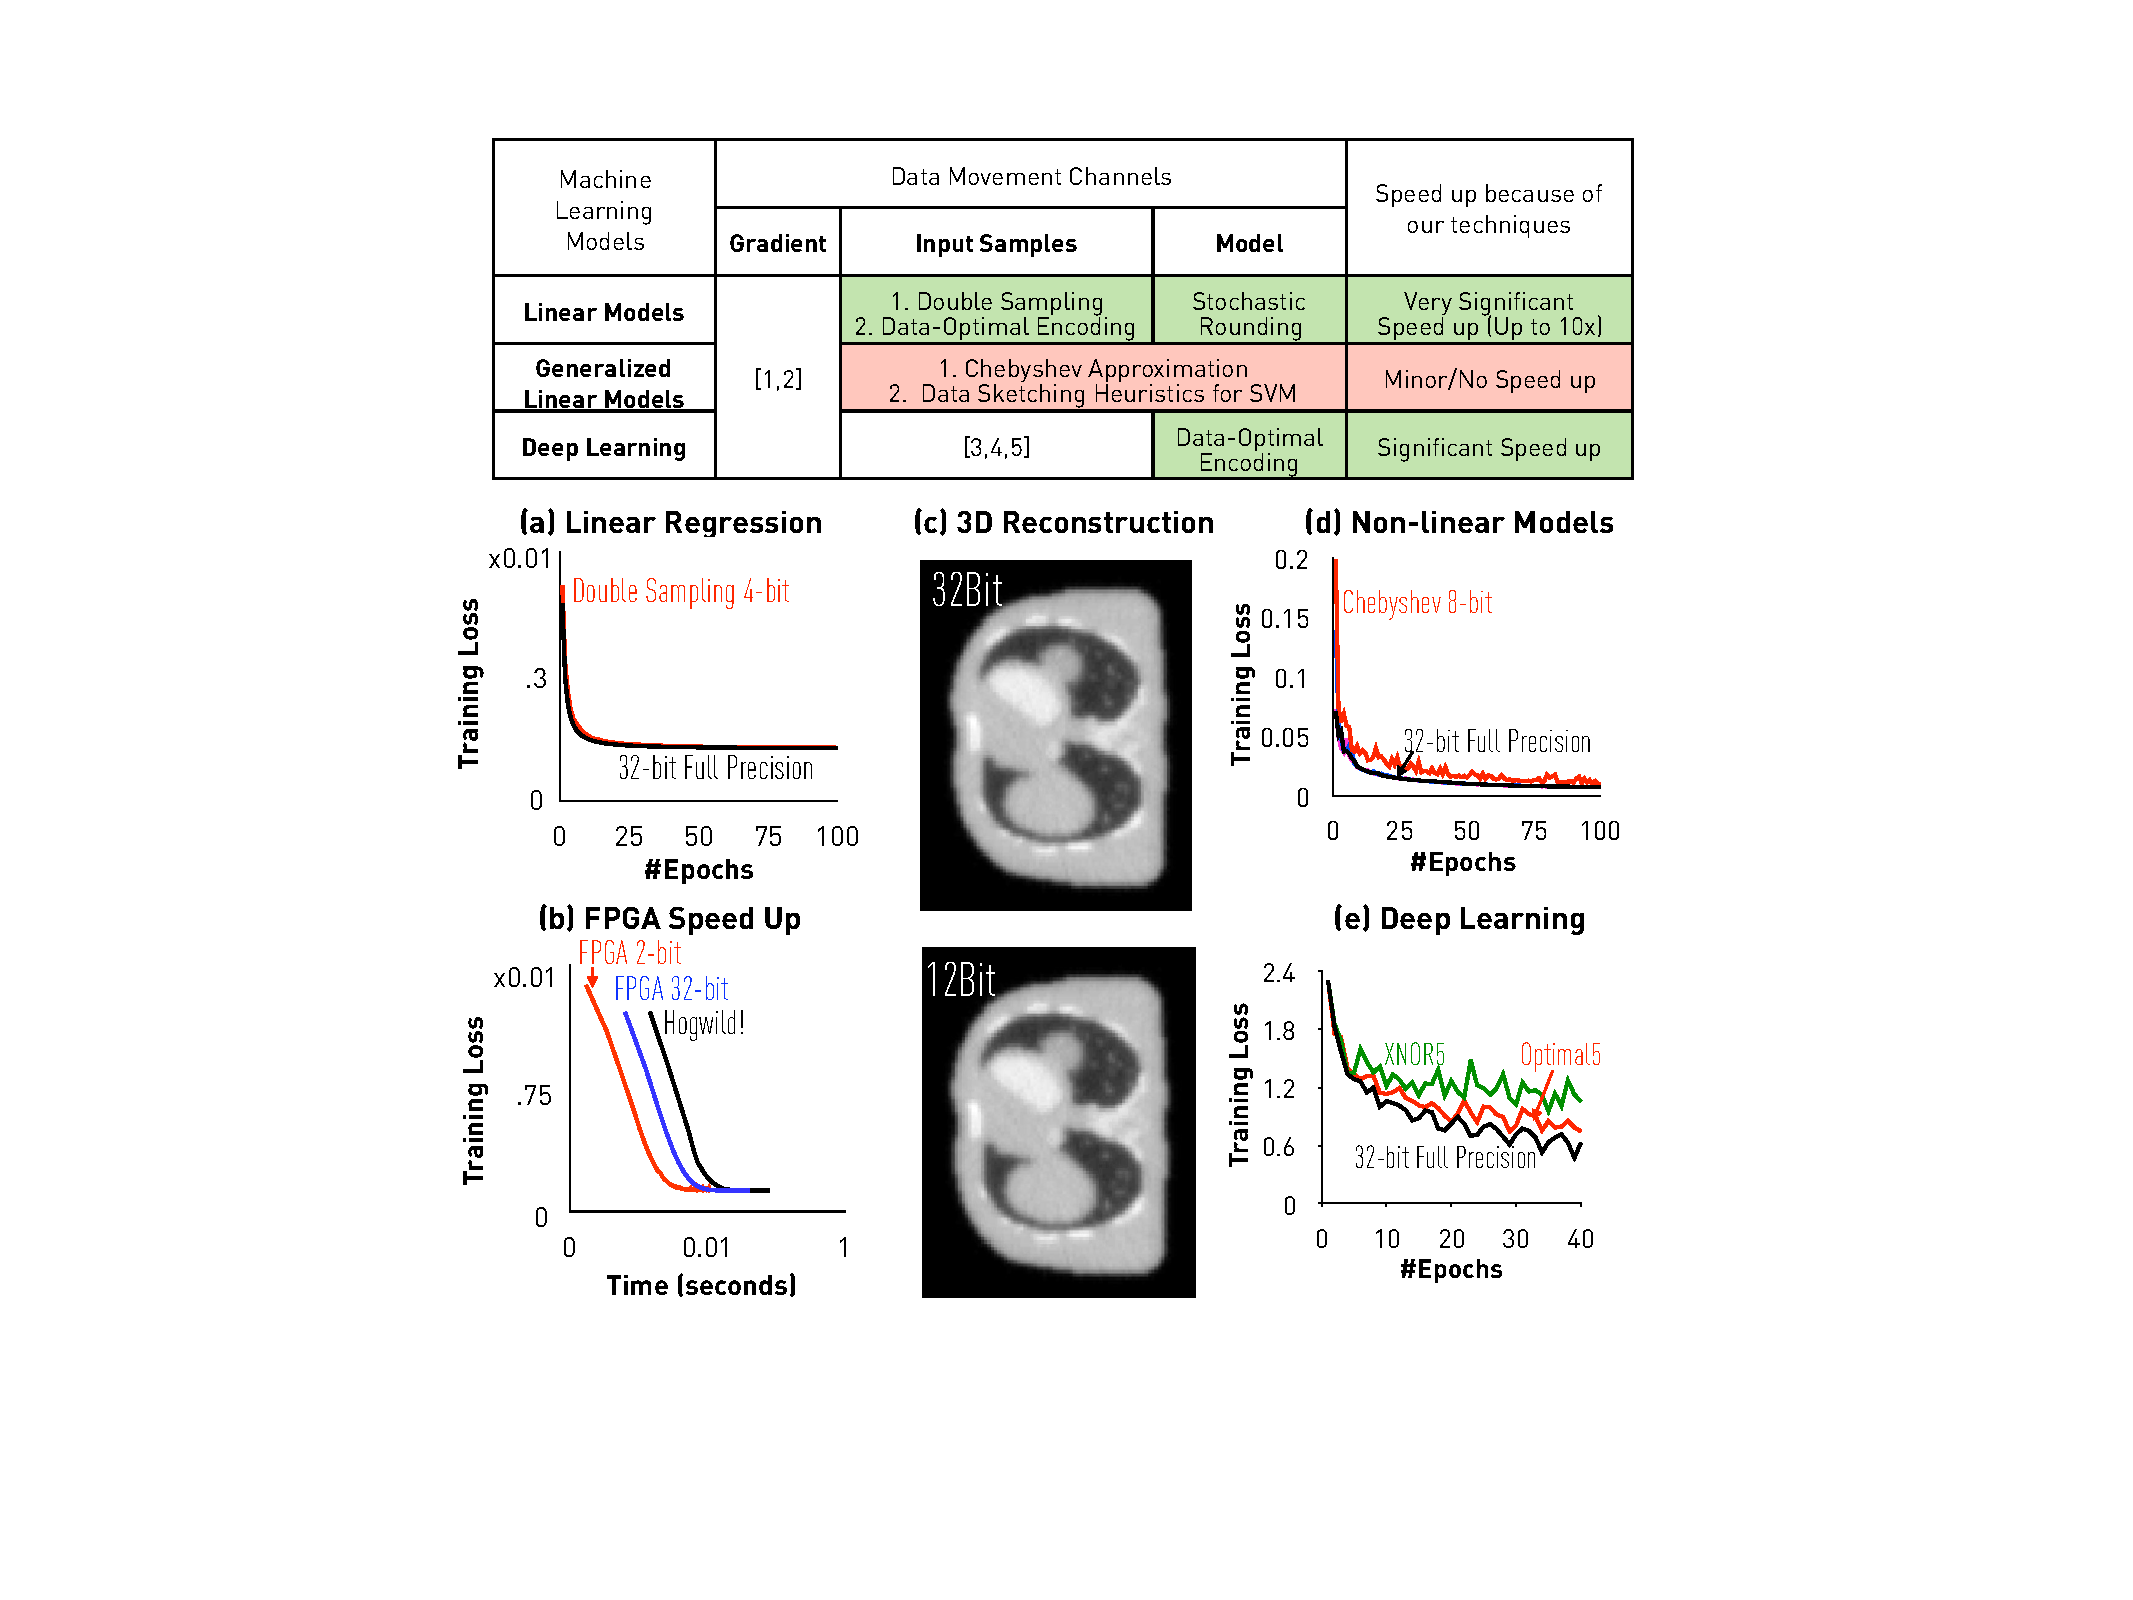
\includegraphics[width=0.5\textwidth]{Figures/RSHighlight}    
\vspace{-2em}
\caption{Overview of theoretical results and
highlights of empirical results. See
Introduction for details.}
\vspace{-1em}
\label{fig:highlight}
\end{figure}

\vspace{-2em}
\section{Introduction}

\vspace{-1em}
The computational cost and power consumption of today's machine learning systems are often driven by data movement, and by the precision of computation. 
In our experience, in applications such as tomographic reconstruction, anomaly detection in mobile sensor networks,
and compressive sensing, the overhead of transmitting the data samples can be massive, 
and hence performance can hinge on reducing the precision of data representation and 
associated computation. 
A similar trend is observed in deep learning, where impressive progress has been reported with systems 
using end-to-end reduced-precision representations~\cite{hubara2016quantized,
rastegari2016xnor,zhou2016dorefa,miyashita2016convolutional}. 
In this context, the motivating question behind our work is:  {\em When training general machine learning models,
can we lower the precision of data representation,
communication, and computation, while maintaining provable guarantees?}
 
% 
%The total operating costs
%or power consumptions of 
%today's machine learning systems 
%are often bounded by data 
%movement and precision of computation.
%From our experience in supporting
%multiple industry partners with 
%a diverse set of applications
%such as tomographic reconstruction,
%anomaly detection over mobile 
%sensor networks, compressive sensing,
%or Ridge regression over
%enterprise data, many of these 
%applications hinge on one question: {\em
%When training generalized linear models,
%can we lower the precision of data representation,
%communication, and computation?}
%
%On the other hand, the Deep Learning
%community has recently witnessed a
%tremendous success in  
%end-to-end low-precision, sometimes as
%low as a single bit, training of neural networks
%with negligible quality loss in many cases~\cite{XXX,XXX,XXX,XXX,
%XXX,XXX,XXX,XXX,XXX}. {\em Can we apply
%these techniques to simpler generalized
%linear models?}

In this paper, we develop a general 
framework to answer this question, and
present both  positive and negative results
 obtained in the context of this framework. 
 Figure~\ref{fig:highlight} encapsulates our results: 
(a) for linear models, we are able to lower the precision of both computation and communication, including input samples, gradients, and model, by up to $16$ times, while still providing rigorous theoretical guarantees; 
(b) our FPGA implementation of this framework achieves up to $6.5\times$ speedup compared with
a 32-bit FPGA implementation, or with a 10-cores CPU running Hogwild!;  
(c) we are able to decrease data movement by $2.7\times$ for
tomographic reconstruction, while getting negligible quality decrease. 
Elements of our framework generalize to (d) non-linear models and  (e) model compression for training deep learning models. 
In the following, we describe our technical contributions in more detail. 


%In this paper, we develop a general 
%framework to answer these questions, and
%present both the positive and negative results
%we obtained. Figure~\ref{fig:highlight} encapsulates our results: 
%(a) for linear
%models, we are able to lower the precision of computation and communication, including input samples, gradients, and model, by up to $16$ times, while still providing rigorous theoretical guarantees 
%we are able to lower the precision of all
%computation and communication involving
%input samples, gradients, and models, by up to 
%$16\times$; (b) when implemented on FPGA, we achieve
%up to $10\times$ speed up compared with
%a 32-bit FPGA implementation and a 10 cores
%CPU running Hogwild!; and (c) we are able to
%decreases data movement by 3$\times$ for
%tomographic reconstruction while getting
%innegligible quality decrease. Our framework
%also applies to (d) non-linear models and 
%(e) model compression for training deep
%learning models. We now summarize our
%technical contributions.

\vspace{-0.5em}
\subsection{Summary of Technical Contributions}

We consider the following problem in training generialized linear models: 
\begin{align}
\min_{\x}:\quad {1\over 2K}\sum_{k=1}^K l(\a_k^\top \x, b_k)^2 + R(\x)
\label{eqn:leastsquares}
\end{align}
where $l(\cdot,\cdot)$ is a loss function, and $R$ is a regularization term, which could be $\ell_1$ norm, $\ell_2$ norm, or even an indicator function representing the constraint. 
The gradient at the sample $(\a_k, b_k)$ is: 
\[
\g_k := \a_k \frac{\partial l(\a_k^\top \x, b_k)}{\partial \a_k^\top \x} 
\]
We denote the problem dimension by $n$. 
We consider the properties of the algorithm when a lossy compression scheme is applied to the data (samples), 
gradient, and model, to reduce the communication cost of the algorithm---that is, we consider quantization functions $Q_g$, $Q_m$, and $Q_s$, for gradient, model and samples, respectively, in the gradient update:
\begin{align}
\x_{t + 1} \leftarrow \text{prox}_{\gamma R(\cdot)}\left(\x_t - \gamma Q_g(\g_k (Q_m(\x_t), Q_s(\vec{a}_t)))\right).
\label{eq:proxupdate}
\end{align}
where the proximal operator is defined as
\[
\text{prox}_{\gamma R(\cdot)}(\y) =\argmin_{\x} {1\over 2}\|\x-\y\|^2 + \gamma R(\x).
\]

%\vspace{-1em}
\paragraph{Our Results} We summarize our results as follows. The {\bf (+)}
sign denotes a ``positive result,'' where we achieve
significant practical speedup, and {\bf (--)} otherwise.

%\vspace{-1em}
\paragraph{(+) Linear Models.} When $l(\cdot,\cdot)$ is 
the least squares loss, we first notice that
simply doing stochastic quantization of data samples  
(i.e., $Q_s$) introduces bias of the gradient
estimator and therefore SGD would converge
to a different solution. We propose a simple
solution to this problem, by introducing a
{\em double sampling} strategy
$\tilde{Q}_s$ that uses multiple samples to
eliminate the correlation of samples introduced
by the non-linearity of the gradient. We
analyze the additional variance introduced
by double sampling, we find that its impact is \emph{negligible in terms of convergence time} as long as the 
number of bits to store a quantized sample is at least $\Theta( \log n / \sigma )$, 
where $\sigma^2$ is the variance of the standard stochastic gradient. 
This implies that the 32 bit precision may be excessive for many practical scenarios. 

We build on this quantization strategy to obtain an \emph{end-to-end quantization} strategy
for linear models, which compresses all data movements. 
For certain settings of parameters, end-to-end quantization adds as little as a \emph{constant factor} to the variance of the entire process. 

%\vspace{-1em}
\paragraph{(+) Optimal Quantization and Extension to Deep Learning.}
We then focus on reducing the variance of  
stochastic quantization. We notice that different ways of setting the quantization points have different variances---the standard uniformly-distributed quantization strategy is far from optimal in many settings.
We formulate this as an independent optimization problem, and solve it optimally with 
an efficient dynamic programming algorithm 
that only need to scan the data in a single pass.
When applied to linear models, this optimal 
strategy can save up to $1.6\times$ communication
compared with the uniform strategy.

We perform an analysis of the optimal quantizations for various settings, and observe that the uniform quantization approach
popularly used by state-of-the-art end-to-end
low-precision deep learning training systems
when more than 1 bit is used is suboptimal.
We apply optimal quantization to 
model quantization and shows that, with one
standard neural network, we outperforms the
uniform quantization used by XNOR-Net and a
range of other recent approaches. This
is related, but different, to recent work 
on model compression for inference~\cite{Han:2016:ICLR}. 
To our best knowledge, this is the first time such optimal quantization strategies have been applied to training. 

%\vspace{-1em}
\paragraph{(--) Non-Linear Models.} We extend our
results to non-linear models such as SVM. We observe that 
we can stretch our multiple-sampling strategy to provide 
unbiased estimators for any polynomials, at the cost of increased variance. 
Building further, we employ Chebyshev polynomials to   
\textcolor{red}{
approximate the gradient of \emph{arbitrary loss functions} within arbitrarily low bias, 
and to provide bounds on the error of an SGD solution obtained from low precision samples. }
%Given the user's error tolerance as input, we can set the bit complexity to lower the bias in order to meet the error threshold. 
%
%By increasing the bit complexity of the representation, we can lower the bias 
%
%This provides a way to control the bias given 
%users' error tolerance as input.  
%When data is separable,
%we prove that \textcolor{red}{BLAH BLAH 
%BLAH BLAH BLAH BLAH BLAH BLAH BLAH BLAH BLAH 
%BLAH BLAH BLAH}. 
In practice, using this technique, we are
able to go as low as 8 bit precision for SVM and logistic regression, \textcolor{red}{while providing 
rigorous theoretical guarantees on the error.} However, we notice that the strawman approach, which just
does naive stochastic rounding over the input data to 8bit precision, converges to similar results in practical settings, 
without the added complexity. 
In a nutshell, this negative result is explained by the fact that, to approximate non-linearities such as the step function or the sigmoid well, our framework needs both high degree Chebyshev polynomials, and relatively large (4bit) samples. 



\vspace{-0.5em}
\section{Linear Models}

%\begin{itemize}
%\item Show the convergence rate of SGD something like
%\[
%f(\x_T) - f^* \leq \Theta\left({L\over T} + {\sum_{t=1}^T \E\|\g_t^{(full)} - \nabla f(\x_t)\|^2/T \over \sqrt{T}}\right) 
%\]
%and emphasize two things: 1) the unbiased stochastic gradient is required for convergence; and 2) the key to improve the convergence is to reduce the variance of stochastic gradient.
%\item Using naive quantization does not work as shown in Section 2.1, since it is biased.
%\item Using the proposed double sampling can ensure unbiased sampling, that is, $\E(\g_t) = \nabla f(\x_t)$ and the stochastic variance of using double sampling can be estimated by
%\begin{align*}
%\E\left[\|\g_t - \nabla f(\x_t)\|^2\right] \leq &\underbrace{\E \|\g_t^{(full)}- \nabla f(\x_t)\|^2}_{\text{from the standard stochastic gradient variance}}
%\\
%&+ \underbrace{\E\|\g_t - \g_t^{(full)}\|^2}_{\text{from the quantization}}
%\end{align*}
%Key point: 1) the first term cannot be avoid and the second term is due to using quantization; 2) in order to not degrade the convergence rate, need to make sure the second term is comparable to the first term. 
%\item Estimate the second term by something like
%\begin{align*}
%&\E\|\g_t - \g_t^{(full)}\|^2 \leq \\
%&\Theta\left(\mathcal{TV}(\a_t) (\mathcal{TV}(\a_t)\|\x\odot \x\| + \|\a_t^\top \x\|^2 + \|\x\odot \x\|\|\a_t\|^2)\right)
%\end{align*}
%where the total variance is 
%\[
%\mathcal{TV}(\a_t) := \E \|Q(\a_t) - \a_t\|^2
%\]
%\item Estimate the upper bound of $\mathcal{TV}(\a_t)$ by something like $n/s^2$ (maybe using uniform quantization), which basically suggests the conclusion in Corollary 1.
%\item In the meantime, we can perform the optimal quantization (not necessarily uniform) to minimize the empirical total variance or mean variance equivalently 
%\[
%\mathcal{TV}(\a_t) = n\mathcal{MV}(\a_t),
%\]
%which is shown in Section 3.
%\end{itemize}


\vspace{-0.5em}
In this section, we focus on linear models with possibly nonsmooth regularization. We have labeled data points $(\a_1, b_1), (\a_2, b_2), \ldots, (\a_K, b_K) \in \R^n \times \R$, and our goal is to minimize the function
\vspace{-0.5em}
\begin{align}
F(\x) = \underbrace{\frac{1}{K} \sum_{k = 1}^K \| \a_k^\top \x - b_k \|_2^2}_{=: f(\x)} + R(\x) \; ,
\label{eq:linear}
\end{align}
i.e., minimize the empirical least squares loss plus a nonsmooth regularization $R(\cdot)$ (e.g., $\ell_1$ norm, $\ell_2$ norm, and constraint indicator function). The generic SGD is the most popular approach to solve the large scale machine learning problem. It works as follows: at step $\x_t$, given an unbiased gradient estimator $\g_t$, that is, 
\[
\E(\g_t) = \nabla f(\x_t)
\]
and update $\x_{t+1}$ by
\[
\x_{t+1} = \text{prox}_{\gamma_t R(\cdot)}\left( \x_t - \gamma_t \g_t\right)
\]
where $\gamma_t$ is the predefined steplength. The generic SGD admits the following convergence property:
\begin{theorem}\label{thm:sgd-conv}[e.g., \cite{2014arXiv1405.4980B}, Theorem 6.3]
Let the sequence $\{\x_t\}_{t=1}^T$ be bounded. Appropriately choosing the steplength,% (e.g., $\gamma_t = 1 / ( L + \sqrt{T})$), 
we have the following convergence rate for \eqref{eq:linear}
% 
%Let $\mathcal{X} \subseteq \R^n$ be convex, and let $f: \mathcal{X} \to \R$ be an unknown, convex, and $L$-smooth. Let $\x_0 \in \mathcal{X}$ be given, and let $R^2 = \sup_{\x \in \mathcal{X}} \| \x - \x_0 \|^2$. Suppose we run projected SGD on $f$ with access to independent stochastic gradients with variance bound $\sigma^2$ for $T$ steps, with step size $\eta_t = 1 / ( L + \gamma^{-1})$, where $\gamma = \frac{R}{\sigma} \sqrt{\frac{2}{T}}$, and
\begin{equation}
F\left(\frac{1}{T} \sum_{t = 0}^T \x_t\right) - \min_{\x}F(\x) \leq \Theta\left({1\over T} + {\sigma \over \sqrt{T}}\right) 
\label{eq:sgd-conv}
%T = O \left( R^2 \cdot \max \left( \frac{2 \sigma^2}{\epsilon^2} , \frac{L}{\epsilon} \right) \right).
\end{equation}
where $\sigma$ is the upper bound of the mean variance 
\[
\sigma^2 \geq {1\over T}\sum_{t=1}^T \E\|\g_t - \nabla f(\x_t)\|^2. 
\]
%Then $\E \left[ f \left( \frac{1}{T} \sum_{t = 0}^T \x_t \right) \right] - \min_{\x \in \mathcal{X}} f(\x) \leq \epsilon$.
\end{theorem} 
\vspace{-0.5em}
There are three key factors to ensure for SGD:
\begin{enumerate}
\vspace{-0.5em}
\item Computing stochastic gradient $\g_t$ is cheap;
\vspace{-0.5em}
\item The stochastic gradient $\g_t$ should be unbiased;
\vspace{-0.5em}
\item The stochastic gradient variance $\sigma$ dominants the convergence efficiency, so it needed to be controlled appropriately.
\end{enumerate}
\vspace{-0.5em}
The common choice is to uniformly select one sample:
\vspace{-0.5em}
\begin{align}
\g_t = \g_t^{(full)} := \a_{\pi(t)} (\a_{\pi(t)}^\top \x - b_{\pi(t)})
\label{eq:sgfull}
\end{align} 
($\pi(t)$ is a uniformly random integer from $1$ to $K$). We abuse the notation and let $\a_t = \a_{\pi(t)}$. Note that $\g_t^{(full)}$ is an unbiased estimator $\E [\g_t^{(full)}] = \nabla f(\x_t)$. Although it has received success in many applications, 
if the precision of sample $\a_{t}$ can be further decreased,
we can save, potentially one order of magnitude, bandwidth
of reading $\a_{t}$ (e.g., in sensor networks) and the associated computation (e.g.,
each register can hold more numbers). 
This motivates us to use low precision sample points to train the model. The following will introduce the proposed low precision SGD framework by meeting all three factors for SGD.


%\paragraph*
\vspace{-0.5em}
\subsection{Stochastic Quantization for Saving Bandwidth} 
\vspace{-0.5em}

We propose to use the stochastic quantization to generate a low precision version of an arbitrary vector $\v$ in the following 
way. Given a vector
$\v$, let $M(\v)$ be a scaling factor such that $-1 \le \v/M(\v) \le 1$. Without loss of generality, let $M(\v)=||\v||_2$. We partition the interval $[-1, 1]$ using $s+1$ separators: $-1 = l_0 \le l_1 ... \le l_{s} = 1$; for each number $v$ in $\v/M(\v)$, we 
quantize it to one of two nearest separators: $l_i \le v \le l_{i+1}$. We denote the \emph{stochastic quantization} function by $Q(\v, s)$ and choose the probability of quantizing to different separators such that $\E[Q(\v, s)] = \v$. We use $Q(\v)$ when $s$ is not relevant.

\vspace{-0.5em}
\subsection{Double Sampling for Unbiased Stochastic Gradient}
\vspace{-0.5em}
%\subsection
%\paragraph{Naive Stochastic Quantization does not Work}
\begin{wrapfigure}{r}{0.23\textwidth}
  \begin{center}
    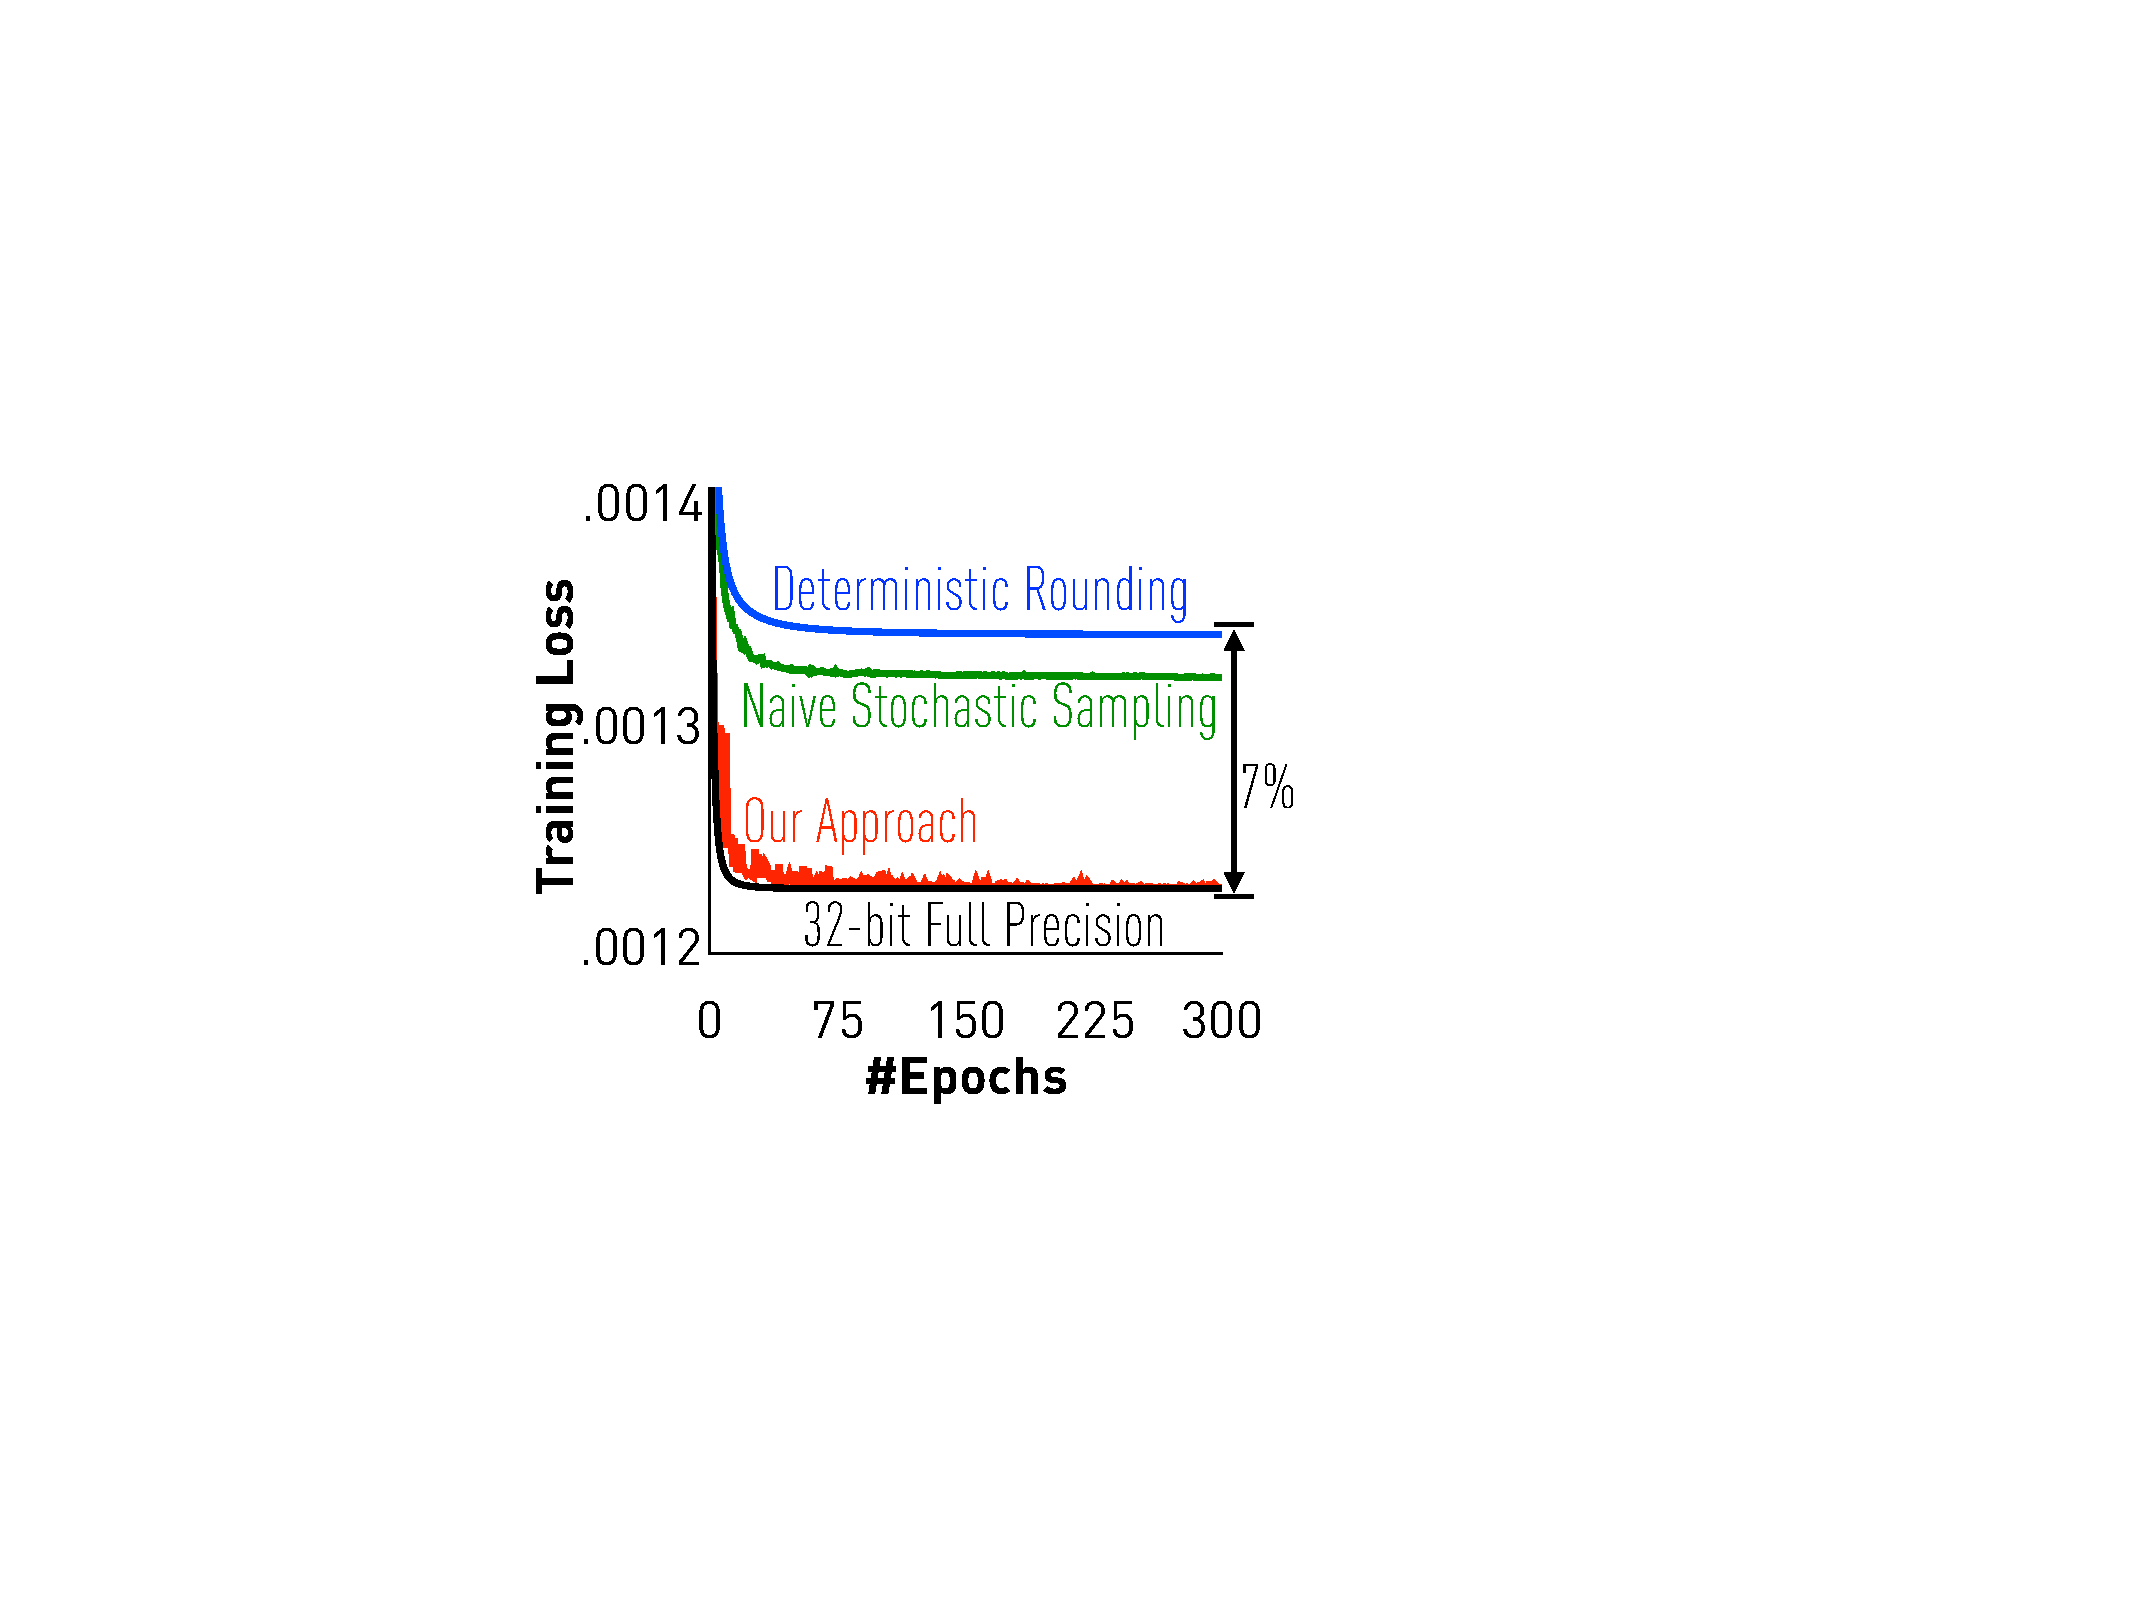
\includegraphics[width=0.23\textwidth]{micro-experiments/gap.pdf}
  \end{center}
  \label{fig:gap}
\end{wrapfigure}
The naive way to use low precision samples $\hat{\a}_t := Q(\a_t)$ is 
\[
\hat{\g}_t := \hat{\a}_t \hat{\a}_t^\top \x - \hat{\a}_t b_t.
\]
However, \emph{the naive way does not work} (even cannot guarantee the convergence), because it is biased: 
\[
\E[\hat{\g}_t] := \a_t \a_t^\top \x - \a_t b_t + D_{\a} \x, 
\]
where $D_{\a}$ is diagonal and its $i$th diagonal element is 
\[
\E[ Q(\a_i)^2 ] - \a_i^2.
\]
%
%\vspace{-0.5em}
%We focus on quantizing the input samples.
%We first establish that, when we quantize $\a_t$
%using the stochastic quantization methods designed
%for gradient, it introduces significant bias.
%Let $\hat{\a}_t = Q(\a_t)$ be the quantized
%sample, the gradient becomes
%\[
%\g_t := \hat{\a}_t \hat{\a}_t^\top \x - \hat{\a}_t b_t.
%\]
%It is not hard to see that the expected gradient is: 
%\[
%\E[\g_t] := \a_t \a_t^\top \x - \a_t b_t + D_{\a} \x, 
%\]
%where $D_{\a}$ is diagonal and its $i$th diagonal element is 
%\[
%\E[ Q(\a_i)^2 ] - \a_i^2.
%\]
%\todo{y axis here is weird}


\vspace{-0.5em}
Since $D_{\a}$ is non-zero, we obtain a \emph{biased} estimator of the gradient, so the iteration is unlikely to converge. 
The figure on the right illustrates the bias caused by a non-zero $D_{\a}$. In fact, it is easy to see that in instances where the minimizer $\x$ is large and gradients become small, we will simply diverge. 

%\vspace{-0.5em}
%\subsection{Double Sampling}
%\vspace{-0.5em}
%\paragraph{Double Sampling}
We now present a simple method to fix the biased gradient estimator. We generate two independent random quantizations and revise the gradient:
\begin{align}
\g_t := Q_1 (\a_t) (Q_2 (\a_t)^\top \x + b_t) \; .
\label{eq:double}
\end{align}
This gives us an unbiased estimator of the gradient $\E(\g_t) = \nabla f(\x)$. 

\paragraph*{Overhead of Storing Two Samples}
Acute readers may notice that one system implication of double sampling is the overhead of sending
two samples instead of one. We note that this will not introduce $2\times$
overhead in terms of data communication, instead, just a single more bit
for the second sample because of the correlation (these two samples 
are only different by at most one bit). More generally, because samples
are used symmetrically, sending $k$ samples only require $\log_2 k$ more bits.

\vspace{-0.5em}
\subsection{Variance Reduction}
\vspace{-0.5em}

From Theorem~\ref{thm:sgd-conv}, the mean variance ${1\over T}\sum_{t}\E\|\g_t - \nabla f(\x)\|^2$ will dominate the convergence efficiency. It is not hard to see that the variance of the double sampling based stochastic gradient in \eqref{eq:double} can be decomposed into
\vspace{-0.5em}
\begin{align*}
\E\|\g_t - \nabla f(\x_t)\|^2 & \leq \E \|\g_t^{(full)}- \nabla f(\x_t)\|^2 
\\
&+ \E \|\g_t - \g_t^{(full)})\|^2
\end{align*}
The first term is from the full stochastic gradient, which can be reduced by using strategies such as mini-batch, weight sampling, etc. How to reduce the first term is an orthogonal issue to this paper. We are more interested in the second term, which is the additional cost for using low precision samples. All strategies of reducing the variance of the first term can seamlessly combine the strategies introduced in this paper, The additional cost can be bounded by
\begin{lemma} 
The stochastic gradient variance using double sampling in \eqref{eq:double} $\E\|\g_t - \g_t^{(full)}\|^2$ can be bounded by
\begin{align*}
%&\E\|\g_t - \g_t^{(full)}\|^2 \leq \\
&\Theta\left(\mathcal{TV}(\a_t) (\mathcal{TV}(\a_t)\|\x\odot \x\| + \|\a_t^\top \x\|^2 + \|\x\odot \x\|\|\a_t\|^2)\right).
\end{align*}
where $\mathcal{TV}(\a_t) := \E\|Q(\a_t) - \a_t\|^2$ and $\odot$ denotes the element product.
\end{lemma}
It suggests that $\mathcal{TV}(\a_t)$ is the key factor to the variance. 

\vspace{-0.5em}
\paragraph{Uniform quantization} Intuitively, more levels of quantization, the lower the variance. The following result shows the quantitative dependence between the variance and the level of quantization with uniform quantization. 
%We assume that these separators are uniformly distributed, and revisit this in Section~\ref{sec:optimal}.
%We have~\cite{Alistarh:2016:ArXiv}: 
\begin{lemma}
\textcolor{red}{
\label{lem:quant-facts} [\cite{Alistarh:2016:ArXiv}]
Assume that these separators are uniformly distributed. For any vector $\vec{v} \in \R^n$, we have that $\E [Q (\vec{v},s)] = \vec{v}$; furthermore, the total variance using uniform quantization with level $s$ is bounded by
\[
\mathcal{TV}_s(\v):=\E [\| Q (\vec{v},s) - \v\|_2^2] \leq \min( n/s^2,\sqrt{n}/s)) \| \vec{v} \|_2^2. \;
\]}
\end{lemma} 

\vspace{-1em}
Together with other results, it suggests the stochastic gradient variance of using double sampling is bounded by
\[
\E\|\g_t - \nabla f(\x_t)\|^2 \leq \sigma^2_{(full)} + \Theta \left( {n /s^2} \right)
\]
where $\sigma^2_{(full)} \geq \E \|\g_t^{(full)} - \nabla f(\x)\|^2$ is the upper bound of using full stochastic gradient, assuming that $\x$ and all $\a_k$'s are bounded. Because the quantization level $s$ is exponential to the number of bits, to ensure these these two terms are comparable (using low precision sample does not degrade the convergence rate), the number of bits only needs to be greater than $\Theta (\log n /\sigma_{(full)})$. We see that even for linear models with millions
of features, 32-bits is likely to be  ``overkill.''

The uniform quantization provides us an intuitive dependence between variance and the level of quantization. However, in practice, we can do better by designing the optimal quantization separation given the quantization level $s$. This motivates
our study in the next section.
 

%\vspace{-0.5em}
%\paragraph{Variance}
%
%Let $r = r(s) = 1 + \min (n / s^2, \sqrt{n}/ s)$ be the blow-up in the second moment because of quantization:
%\begin{lemma}
%\label{lem:qbound}
%    Given $\a_k, \x, b_k$, suppose $\| \a_k \|_2^2 \leq A^2, \| \x \|_2^2 \leq R^2$ and $\max_i |\a_k| \leq M_a$.
%    Let $\g_k^{(full)}$ be the unquantized stochastic gradient. We have
%    \[
%    \E_{Q_1, Q_2} [\| \g_k \|_2^2] \leq r \cdot \left( \| \g_k^{(full)} \|_2^2 \cdot \frac{M_a^2}{\| \a_k \|_2^2} + \frac{A^2 M_a^2 R^2}{s^2} \right)\; .
%    \]
%\end{lemma}
%
%This implies the following variance bound:
%\begin{corollary}
%    Let $\a_k, \x, b_k, \g_k^{(full)}$ be as above.
%    Suppose $\E [\| \g_k^{(full)} - \nabla f(\x_k) \|_2^2 ] \leq \sigma^2$ and $\E [\| \g_k^{(full)} \|_2^2] \leq B$. We have
%    \[
%    \E \left[ \| \g_k - \nabla f(\x_k) \|_2^2 \right] \leq  \sigma^2 + \left(r \frac{M_a^2}{\| \a_k \|_2^2} - 1\right) B + \frac{r A^2 M_a^2 R^2}{s^2} \; ,
%    \]
%    where the expectation is taken over $\g_k^{(full)}$ and the randomness of the quantization.
%\end{corollary}
%
%This corollary suggests that the quantized stochastic gradient variance is bounded by
%\[
%\E \left[ \| \g_k - \nabla f(\x_k) \|_2^2 \right] \leq \sigma^2 + \Theta(n/s^2) \;
%\]
%in the scenario when $M_i (\vec{v}) = \| \vec{v} \|_2 $.
%The first term $\sigma^2$ is introduced by stochastic gradient, while the second term is introduced by quantization. Because the value of $s$ is 
%exponential to the number of bits, to ensure these two terms are comparable (to maintain the same convergence rate), the number of bits needs to be greater than $\Theta(\log n / \sigma)$. We see that even for linear models with millions
%of features, 32-bits is likely to be  ``overkill.''
%
%
%
%\vspace{-0.5em}
%\paragraph*{Overhead of Storing Two Samples}
%One system implication of double sampling is the overhead of sending
%two samples instead of one. We note that this will not introduce $2\times$
%overhead in terms of data communication, instead, just a single more bit
%for the second sample because of the correlation (these two samples 
%are only different by at most one bit). More generally, because samples
%are used symmetrically, sending $k$ samples only require $\log_2 k$ more bits.
%
%\vspace{-0.5em}
%\paragraph*{Extensions}
%
%All of our results can be applied to 
% problems 
%with possibly non-smooth regularization term. The key substitution is to use the proximal update defined in \eqref{eq:proxupdate}.
%Also, extending our result to least-squares SVMs for classification is trivial~\cite{Suykens:1999:Book}.
%We leave these details to the full version
%of this paper.
%
%\vspace{-0.5em}
%\subsection{End-to-end Quantization}
%\vspace{-0.5em}
%
%We can now develop an end-to-end quantization strategy that
%quantizes gradients, model, and input samples all 
%at the same time. The gradient becomes:
%\[
%\g_k := Q_1 \left( Q_2(\a_k, s ) ( Q_3(\a_k, s)^\top Q_4(\x, s) + b_k) , s \right),
%\]
%\noindent 
%where all $Q$'s are independent quantizations.
%
%%  $Q_3$ and 
%%The iteration becomes: 
%%
%%\begin{eqnarray}
%%	\x = \x - \gamma \g_k.
%%\end{eqnarray}
%
%\noindent From combining the previous results, we have:
%
%\begin{corollary}
%    \label{cor:full-quantization}
%    Let $\a_k, \x, b_k$ be so that $\| \a_k \|_2^2 \leq 1, \| \x \|_2^2 \leq R^2$.
%    Let $M_a, M_x$ be as above, and let $\g_k^{(full)}$ be the (unquantized) stochastic gradient.
%    We have
%    \[
%    \E [\| \g_k \|_2^2] \leq r^2 M_a \cdot \left(  \| \g_k^{(full)} \|_2^2 + \frac{R^2}{s^2}   + \frac{r M_a R^2}{s^2} \right) \; .
%    \]
%\end{corollary}





%\vspace{-0.5em}
In this section, we focus on linear models.
We have labeled data points $(\a_1, b_1), (\a_2, b_2), \ldots, (\a_K, b_K) \in \R^n \times \R$, and our goal is to minimize the function
\[
f(\x) = \frac{1}{K} \sum_{k = 1}^K \| \a_k^\top \x - b_k \|_2^2 \; ,
\]
i.e., minimize the empirical least squares loss.
The full-precision SGD works as 
follows: at step $\x_k$, our gradient estimator is $\g_k^{(full)} = \a_{\pi(k)} (\a_{\pi(k)}^\top \x - b_{\pi(k)})$, where $\pi(k)$ is a uniformly random integer from $1$ to $K$.
We abuse the notation and let $\a_k = \a_{\pi(k)}$.
We have $\E [\g_k^{(full)}] = \nabla f(\x_k)$.

\vspace{-1em}
\paragraph*{Stochastic Quantization} 
Given a vector
$\v$, let $M(\v)$ be a scaling factor such that
$-1 \le \v/M(\v) \le 1$. Without loss of generality,
let $M(\v)=||\v||_2$. We partition
the interval $[-1, 1]$ using $s+1$ separators:
$-1 = l_0 \le l_1 ... \le l_{s} = 1$; for
each number $v$ in $\v/M(\v)$, we 
quantize it to one of two nearest 
separators: $l_i \le v \le l_{i+1}$. 
We denote the \emph{stochastic quantization} function by $Q(\v, s)$
and choose the probability of quantizing to
different separators such that $\E[Q(\v, s)] = \v$.
We use $Q(\v)$ when $s$ is not relevant.
We assume that these
separators are uniformly distributed,
and revisit this in Section~\ref{sec:optimal}.
We have~\cite{Alistarh:2016:ArXiv}: 
\begin{lemma}
\label{lem:quant-facts}
For any vector $\vec{v} \in \R^n$, we have that $\E [Q (\vec{v},s)] = \vec{v}$, and furthermore, we have
$
\E [\| Q (\vec{v},s) \|_2^2] \leq (1 + \min( n/s^2,\sqrt{n}/s)) \| \vec{v} \|_2^2 \; .
$
\end{lemma} 




\vspace{-0.5em}
\subsection{Naive Stochastic Quantization is Biased}

\vspace{-0.5em}
We focus on quantizing the input samples.
We first establish that, when we quantize $\a_k$
using the stochastic quantization methods designed
for gradient, it introduces significant bias.
Let $\hat{\a_k} = Q(\a_k)$ be the quantized
sample, the gradient becomes
\[
\g_k := \hat{\a_k} \hat{\a_k}^\top \x - \hat{\a_k} b_k.
\]
It is not hard to see that the expected gradient is: 
\[
\E[\g_k] := \a_k \a_k^\top \x - \a_k b_k + D_{\a} \x, 
\]
where $D_{\a}$ is diagonal and its $i$th diagonal element is 
\[
\E[ Q(\a_i)^2 ] - \a_i^2.
\]

%\todo{y axis here is weird}
\begin{wrapfigure}{r}{0.23\textwidth}
  \begin{center}
    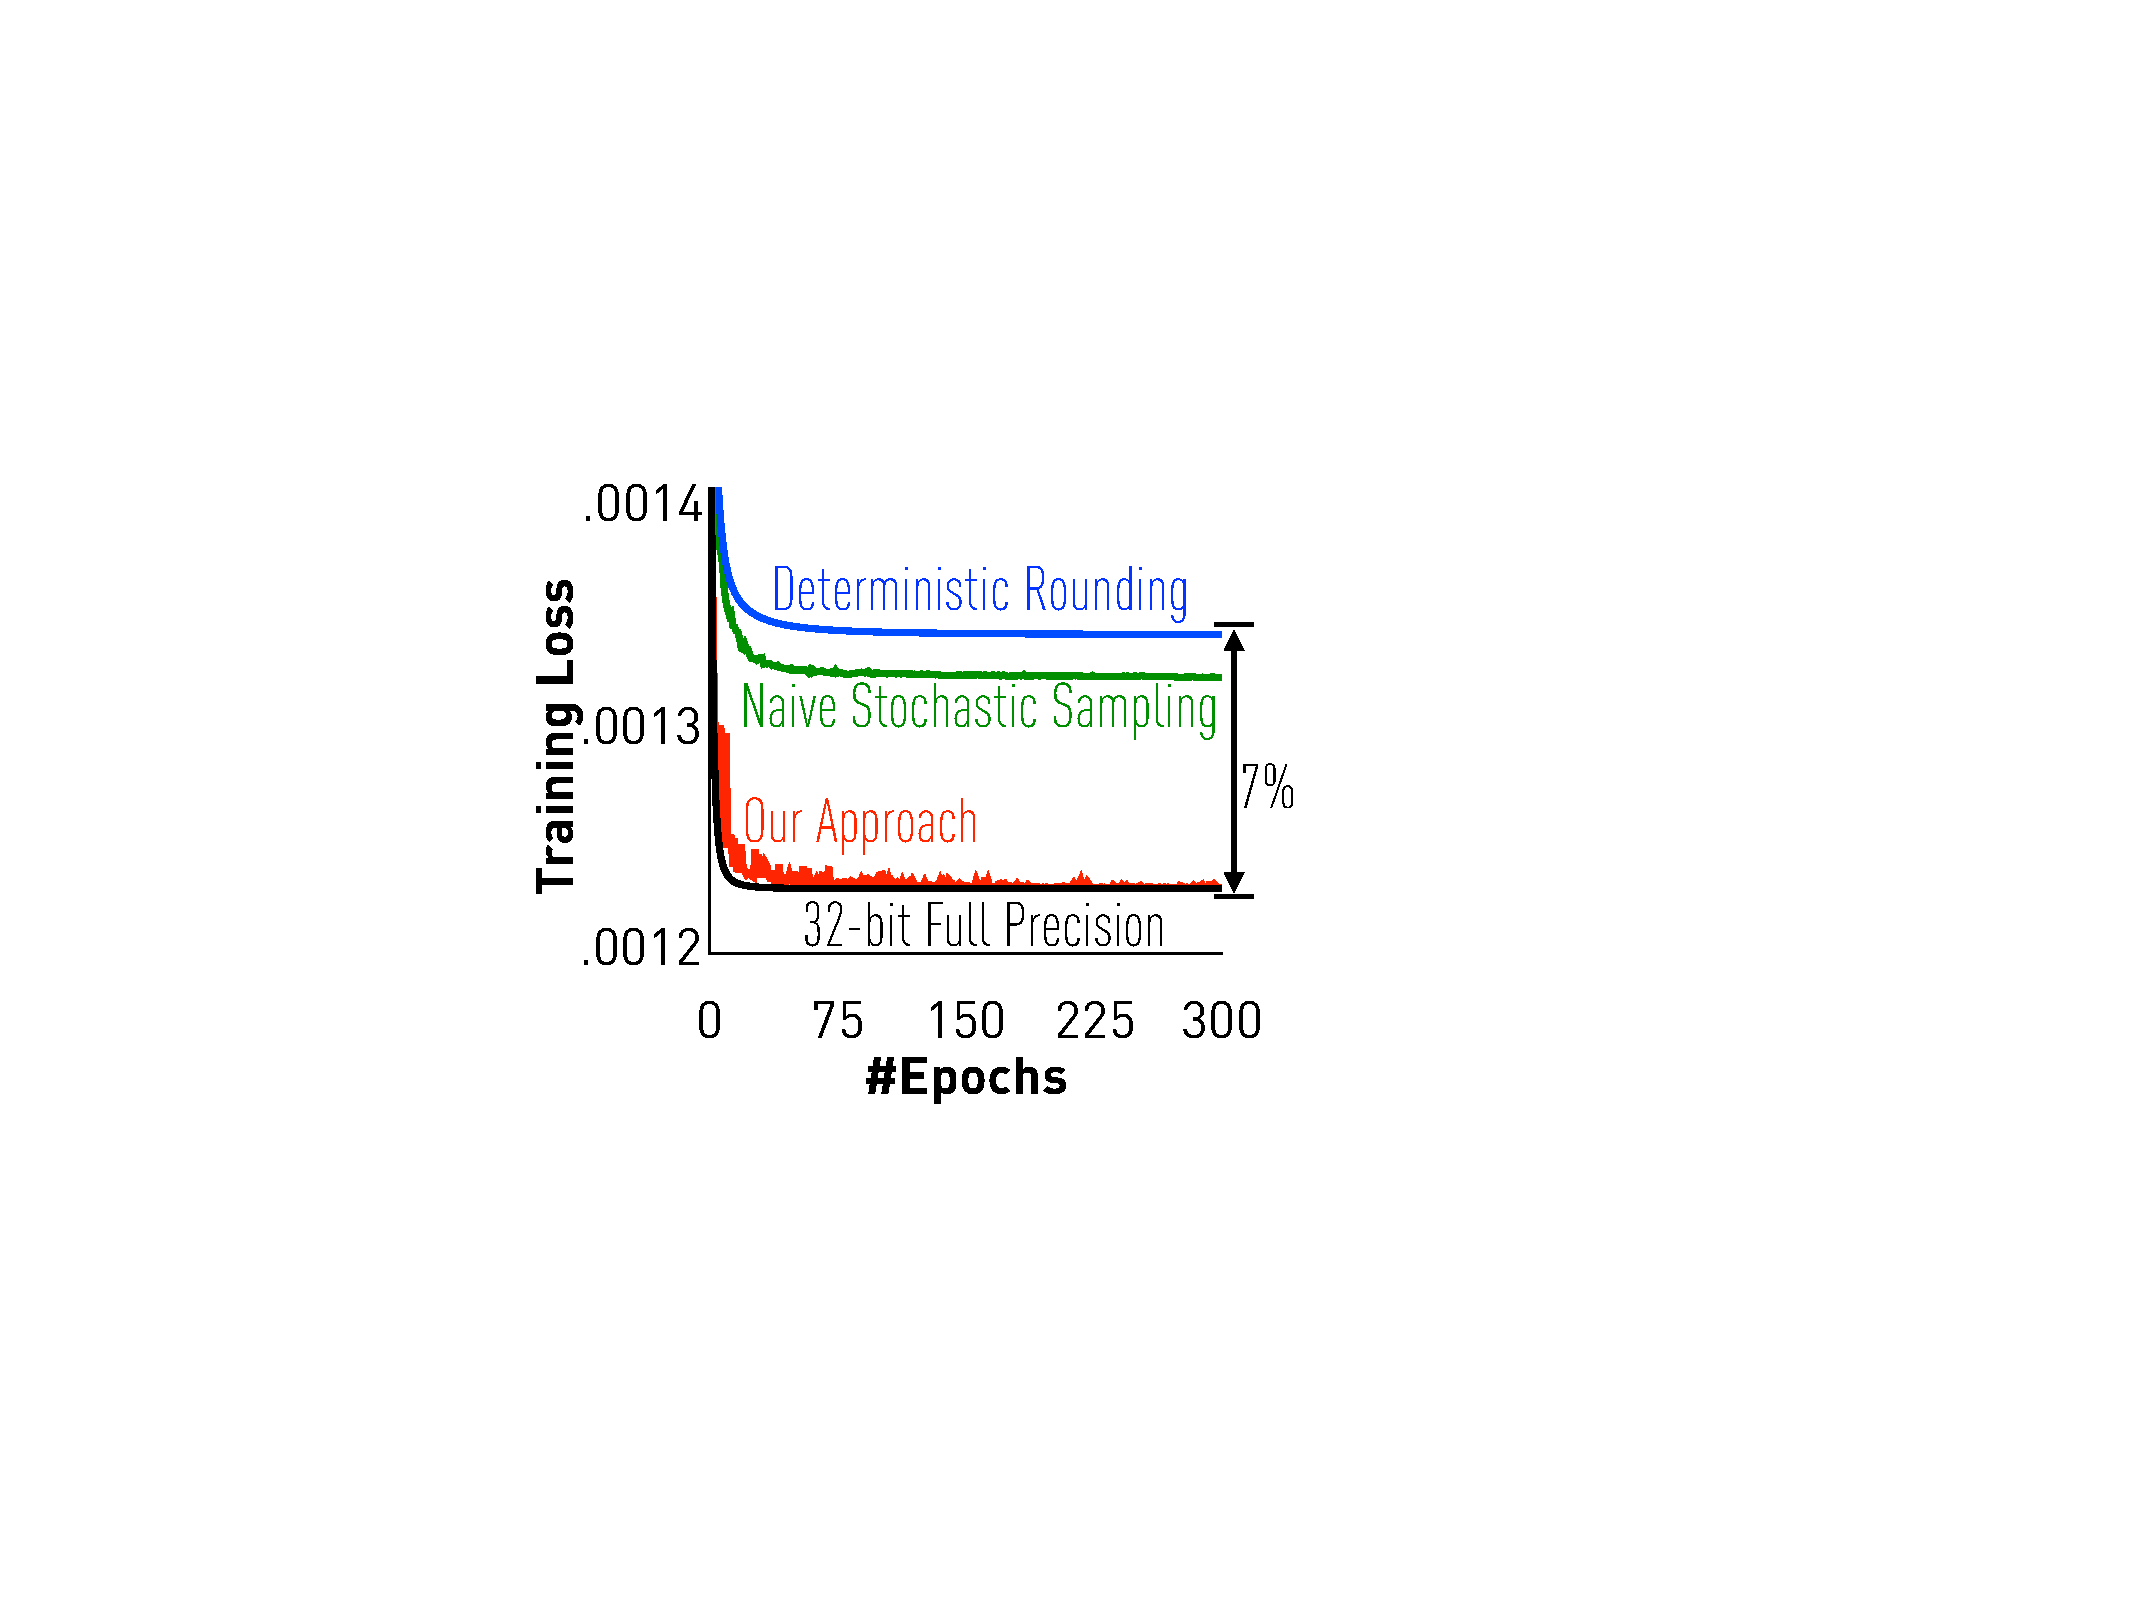
\includegraphics[width=0.23\textwidth]{micro-experiments/gap.pdf}
  \end{center}
  \label{fig:gap}
\end{wrapfigure}

\vspace{-0.5em}
Since $D_{\a}$ is non-zero, we obtain a \emph{biased} estimator of the gradient, so the iteration is unlikely to converge. 
The figure on the right illustrates the bias
caused by a non-zero $D_{\a}$.
In fact, it is easy to see that in instances where the minimizer $\x$ is large and gradients become small, we will simply diverge. 

\vspace{-0.5em}
\subsection{Double Sampling}
\vspace{-0.5em}

We now present a simple method to fix the biased gradient estimator.
We generate two independent
random quantizations and revise the gradient:
\[
\g_k := Q_1 (\a_k) (Q_2 (\a_k)^\top \x + b_k) \; .
\]
This gives us an unbiased estimator 
of the gradient.

\vspace{-0.5em}
\paragraph{Variance}

Let $r = r(s) = 1 + \min (n / s^2, \sqrt{n}/ s)$ be the blow-up in the second moment because of quantization:
\begin{lemma}
\label{lem:qbound}
    Given $\a_k, \x, b_k$, suppose $\| \a_k \|_2^2 \leq A^2, \| \x \|_2^2 \leq R^2$ and $\max_i |\a_k| \leq M_a$.
    Let $\g_k^{(full)}$ be the unquantized stochastic gradient. We have
    \[
    \E_{Q_1, Q_2} [\| \g_k \|_2^2] \leq r \cdot \left( \| \g_k^{(full)} \|_2^2 \cdot \frac{M_a^2}{\| \a_k \|_2^2} + \frac{A^2 M_a^2 R^2}{s^2} \right)\; .
    \]
\end{lemma}

This implies the following variance bound:
\begin{corollary}
    Let $\a_k, \x, b_k, \g_k^{(full)}$ be as above.
    Suppose $\E [\| \g_k^{(full)} - \nabla f(\x_k) \|_2^2 ] \leq \sigma^2$ and $\E [\| \g_k^{(full)} \|_2^2] \leq B$. We have
    \[
    \E \left[ \| \g_k - \nabla f(\x_k) \|_2^2 \right] \leq  \sigma^2 + \left(r \frac{M_a^2}{\| \a_k \|_2^2} - 1\right) B + \frac{r A^2 M_a^2 R^2}{s^2} \; ,
    \]
    where the expectation is taken over $\g_k^{(full)}$ and the randomness of the quantization.
\end{corollary}

This corollary suggests that the quantized stochastic gradient variance is bounded by
\[
\E \left[ \| \g_k - \nabla f(\x_k) \|_2^2 \right] \leq \sigma^2 + \Theta(n/s^2) \;
\]
in the scenario when $M_i (\vec{v}) = \| \vec{v} \|_2 $.
The first term $\sigma^2$ is introduced by stochastic gradient, while the second term is introduced by quantization. Because the value of $s$ is 
exponential to the number of bits, to ensure these two terms are comparable (to maintain the same convergence rate), the number of bits needs to be greater than $\Theta(\log n / \sigma)$. We see that even for linear models with millions
of features, 32-bits is likely to be  ``overkill.''

\vspace{-0.5em}
\paragraph*{Overhead of Storing Two Samples}
One system implication of double sampling is the overhead of sending
two samples instead of one. We note that this will not introduce $2\times$
overhead in terms of data communication, instead, just a single more bit
for the second sample because of the correlation (these two samples 
are only different by at most one bit). More generally, because samples
are used symmetrically, sending $k$ samples only require $\log_2 k$ more bits.

\vspace{-0.5em}
\paragraph*{Extensions}

All of our results can be applied to 
 problems 
with possibly non-smooth regularization term. The key substitution is to use the proximal update defined in \eqref{eq:proxupdate}.
Also, extending our result to least-squares SVMs for classification is trivial~\cite{Suykens:1999:Book}.
We leave these details to the full version
of this paper.

\vspace{-0.5em}
\subsection{End-to-end Quantization}
\vspace{-0.5em}

We can now develop an end-to-end quantization strategy that
quantizes gradients, model, and input samples all 
at the same time. The gradient becomes:
\[
\g_k := Q_1 \left( Q_2(\a_k, s ) ( Q_3(\a_k, s)^\top Q_4(\x, s) + b_k) , s \right),
\]
\noindent 
where all $Q$'s are independent quantizations.

%  $Q_3$ and 
%The iteration becomes: 
%
%\begin{eqnarray}
%	\x = \x - \gamma \g_k.
%\end{eqnarray}

\noindent From combining the previous results, we have:

\begin{corollary}
    \label{cor:full-quantization}
    Let $\a_k, \x, b_k$ be so that $\| \a_k \|_2^2 \leq 1, \| \x \|_2^2 \leq R^2$.
    Let $M_a, M_x$ be as above, and let $\g_k^{(full)}$ be the (unquantized) stochastic gradient.
    We have
    \[
    \E [\| \g_k \|_2^2] \leq r^2 M_a \cdot \left(  \| \g_k^{(full)} \|_2^2 + \frac{R^2}{s^2}   + \frac{r M_a R^2}{s^2} \right) \; .
    \]
\end{corollary}






\vspace{-2em}
\section{Optimal Quantization Strategy} \label{sec:optimal}

\vspace{-0.5em}
We now revisit the choice of quantization points
and present an optimal strategy to minimize 
the variance term introduced by quantization.

Give a set of real numbers $\Omega$ with cardinality $N$ and allowed $K$ level quantization. Without the loss of generality, we assume that all real numbers in $\Omega$ is in $[0, 1]$. The goal is to decide the optimal $K$ quantization levels $\{p_1, p_2, \cdots, p_{K-1}\}$ for this set to minimize the overall variance
\begin{align}
\min_{0\leq p_1\leq p_2 \leq \cdots \leq p_{K-1} \leq 1}\quad \sum_{x\in \Omega} \sum_{k=1}^K {\bf 1}_k(x)V_k(x)
\end{align}
where ${\bf 1}_k(x)$ is the indicator function
\[
{\bf 1}_k(x) = 
\begin{cases}
1 & \text{if}~x\in (p_{k-1}, p_k] \\
0 & \text{o.w.}
\end{cases}
\]
with $p_0=0$ and $p_K=1$, and the $V_k(x)$ is the variance function 
\[
V_k(x) = (x-p_{k-1})(p_k - x), 
\]
which is the variance of Bernoulli distribution with probability $p_k-x$ taking value $p_{k-1}$ and probability $x-p_{k-1}$ taking value $p_k$. ${\bf 1}_k(x)V_k(x)$ is the variance if $x$ falls into the interval $(p_{k-1}, p_k]$. 

This problem is hard to solve directly due to the non-convexity and non-smoothness. We discretize the range $[0,1]$ into $M$ internals, that is, $[0,d_1), [d_1, d_2), \cdots, [d_{M-1}, 1]$ with $0< d_1<d_2<\cdots < d_{M-1}<1$. All $p_k$'s can only take the values in $\{d_1, d_2, \cdots, d_{M-1}\}$ while satisfy the monotonicity.

Define $T(k, m)$ be the optimal total variance for points in $[0, d_m]$ with $k$ quantization levels. Our goal is to calculate $T(K, M)$. This problem can be solved by dynamic programing using the following recursion
\[
T(k, m) = \min_{j\in \{k-1, k, \cdots, m-1\}} T(k-1,j) + V(j,m)
\]
where $V(j,m)$ is the total variance of points falling into the interval $[d_j, d_m]$. The optimal value for $p_{K-1}^*$ is $ d_{j^*_{K-1}}$ with $j^*_{K-1}$ equal to
\[
j^*_{K-1} = \argmin_{j\in \{K-1, k, \cdots, M-1\}} T(K-1,j) + V(j,M),
\]
and the rest can be retrieved by 
\begin{align*}
j^*_{k-1} = \argmin_{j\in \{k-1, k, \cdots, j^*_k-1\}} T(k-1, j) + V(j, j^*_k) \\
\text{for all}~k=2, \cdots, K-2
\end{align*}

The complexity of calculating matrix $V(\cdot, \cdot)$ is $O(M^2 + N)$ and the complexity of calculating matrix $T(\cdot, \cdot)$ is $O(KM^2)$. The total memory cost is $O(KM + M^2)$.

\vspace{-0.5em}
\subsection{Extension to Deep Learning}
\vspace{-0.5em}

In this section, we show that it is possible 
to apply optimal quantization to
training deep neural networks.

\paragraph*{State-of-the-art} We focus on
training deep neural networks with quantized
model. Let $\mathcal{W}$ be the model and 
$l(\mathcal{W})$ be the loss function. State-of-the-art quantized networks,
such as XNOR-Net and QNN, replace $\mathcal{W}$
with the quantized version $Q(\mathcal{W})$, and optimize
for
\[
\min_{\mathcal{W}} l(Q(\mathcal{W})).
\]
With a properly defined 
$\frac{\partial Q}{\partial{\mathcal{W}}}$, we can
apply the standard backprop 
algorithm.

Choosing the quantization function $Q$ is
an important design decision. For 1-bit quantization,
XNOR-Net searches the optimal quantization point. However, for multiple bits,
XNOR-Net, as well as other approaches such as QNN, resort
to uniform quantization.

\vspace{-0.5em}
\paragraph*{Optimal Model Quantization for Deep Learning}

We can apply our optimal quantization strategy 
and use it as the quantization function $Q$
in XNOR-Net. Empirically, this results in 
quality improvement
over with the default {\em multi-bits} quantizer in XNOR-Net. 

In spirit, our approach is similar to the 1-bit quantizer of
XNOR-Net, which is equivalent to our approach when the data
distribution is symmetric---we extend this
to multiple bits in a principled way. Another related work
is the uniform quantization strategy 
in {\em log domain}~\cite{miyashita2016convolutional},
which is similar to our approach when the data distribution
is ``log uniform''. However, our approach does not rely on
any specific assumption of the data distribution.
\citet{Han:2016:ICLR} use $k$-means to
compress the model for {\em inference}~---$k$-means
optimizes for a similar, but different, objective
function than us. In this paper, we 
develop a dynamic
programming algorithm to do optimal quantization efficiently,
and to our best knowledge, we
are the first to apply optimal quantization to
{\em training}.



%!TEX root = main.tex
\section{Non-Linear Models}

In this section, we extend our framework to approximate arbitrary classification losses within arbitrarily small bias. 
Although theoretically justified, this framework can become heavyweight for loss functions which are not well approximable by polynomials 
(e.g., hinge). We provide efficient quantization heuristics for these loss functions. 

\subsection{Quantizing Arbitrary Polynomials} 

Assume we are given a degree $d$ polynomial $P(x) = \sum_{i = 0}^{d} m_i z^i$, and that 
we wish to evaluate it at $\vec{a}^\top \vec{x}$, while quantizing $\vec{a}$, so as to preserve the value of $P( \vec{a}^\top \vec{x})$ in expectation. 
We do so as follows. 

We will use $d$ independent quantizations of $\vec{a}$, $Q_1(\vec{a}), Q_2(\vec{a}), \ldots, Q_d(\vec{a})$. 
Given these quantizations, our reconstruction of the polynomial will be 
$$ Q(P) := \sum_{i = 0}^d m_i \prod_{j \leq i} Q_j(\vec{a})^\top \vec{x}.$$

The fact that this is an unbiased estimator of $P( \vec{a}^\top \vec{x} )$ follows from the independence of the quantizations. Extending the analysis in Lemma~\ref{lem:qbound} yields:

\begin{lemma}
\label{lem:poly-sec-moment-bound}
	$\E[ Q(P)^2 ] \leq 2^d \sum_{i = 0}^d m_i r(s)^i (\vec{a}^\top \vec{x})^i.$
\end{lemma} 








\subsection{Quantizing Arbitrary Classification Losses}

Assume a standard classification setting, where we have samples $[(\vec{a}_i, b_i)]_i$ drawn from a distribution $\mathcal{D}$, a loss function $\ell: \R \rightarrow \R$, and we wish to find $\vec{x}$ which minimizes $\E_{\mathcal{D}} [ \ell( b \cdot \vec{a}^\top \vec{x} ]$. The gradient of $\ell$ is given by 
$$ \nabla_\vec{x} (b \cdot \vec{a}^\top \vec{x}) = b \ell' (b \cdot \vec{a}^\top \vec{x}) \vec{a}.$$

Assume normalized samples, i.e. $\| \vec{a}_i \|_2 \leq 1, \forall i$, and that $\vec{x}$ is constrained such that $\| \vec{x} \|_2 \leq R$, for some real value $R > 0$. We are given a target accuracy $\epsilon$, within which we wish to approximate the gradient. 

Given this, we fix the minimal-degree polynomial $P$ such that $|P(z) - \ell'(z)| \leq \epsilon, \forall z \leq R$. This polynomial is known to both transmitter (sample source) and receiver (compute device). The protocol is as follows. 
\begin{itemize}
	\item For a given sample $(\vec{a}_i, b_i)$ to be quantized, the source will transmit $b_i$, as well as $d + 1$ independent quantizations $Q_1, Q_2, \ldots, Q_{d + 1}$ of $\vec{a}_i$. 
	\item The receiver computes $b \cdot Q(P) Q_{d + 1} ( \vec{a}_i )$ and uses it as the gradient.
\end{itemize}

It is easy to see that the bias in each step is bounded by $\epsilon$. 
We can extend Lemma~\ref{lem:poly-sec-moment-bound} to obtain a general bound on convergence. 

\begin{lemma}
	\textcolor{red}{DAN: TODO here}
\end{lemma}

\paragraph{Chebyshev Approximations} 
For \emph{hinge loss}, the gradient is the step function, which is hard to approximate generally by polynomials. 
However, the problem is well studied for intervals of the type  $[-R, R] \setminus [-\delta, \delta]$, for some small parameter $\delta > 0$~\cite{frostig2016principal, allen2016faster}; the latter reference provides the optimal approximation via Chebyshev polynomials, which we use in our experiments. 

For \emph{logistic loss}, with sigmoid gradient, we again notice that polynomial approximations have been well studied. In particular, we use the optimal Chebyshev polynomial approximation of~\cite{vlcek2012chebyshev}. 

\paragraph{Practical Considerations} The above strategy introduces a precision-variance trade-off, since increasing the precision of approximation (higher polynomial degree) also increases the variance of the gradient. 
Fortunately, we can further reduce the variance and increase the approximation quality by increasing the density of the quantization. 
The results in Section~\ref{sec:exp} show that a total of $8$ bits per sample is sufficient to ensure convergence to the same result as the full-precision 
implementation for both hinge loss and logistic loss. 




%\textcolor{red}{DAN: ADD ONE SENTENCE ABOUT HOW IT WORKS IN PRACTICE?}



\begin{table}[t]
\scriptsize
\centering
\begin{tabular}{crrrr}
\hline
\multicolumn{4}{c}{\bf Regression}\\
Dataset           & Training Set & Testing Set & \# Features  \\
\hline
Synthetic 10   & 10,000        & 10,000       & 10               \\
Synthetic 100  & 10,000        & 10,000       & 100              \\
Synthetic 1000 & 10,000        & 10,000       & 1,000           \\
YearPrediction & 463,715       & 51,630       & 90                  \\
cadata         & 10,000        & 10,640       & 8                   \\
cpusmall       & 6,000         & 2,192        & 12     \\
\hline
\hline
\multicolumn{4}{c}{\bf Classification}\\
Dataset           & Training Set & Testing Set & \# Features \\
\hline
cod-rna        & 59,535        & 271,617      & 8    \\
gisette        & 6,000         & 1,000        & 5,000  \\  
epsilon        & 10,000        & 10,000       & 2,000\\  
\hline
\hline
\multicolumn{4}{c}{\bf Deep Learning}\\
Dataset           & Training Set & Testing Set & \# Features \\
\hline
CIFAR-10        & 50,000        & 10,000      &$32\times 32\times 3$     \\
\hline
\end{tabular}
\caption{Dataset statistics}
\label{table:dataset}
\end{table}

\vspace{-0.5em}
\section{Experiments} \label{sec:exp}

\vspace{-0.5em}
We provide empirical validation of
our framework on a range of
models, including
(1) linear models, (2) non-linear models,
and (3) deep learning.

\vspace{-1em}
\paragraph{Experimental Setup} 
Table~\ref{table:dataset} shows the 
datasets we use. 
Unless otherwise noted, we always
use diminishing stepsizes $\alpha/k$
where $k$ is the current number of
epoch. We tune 
$\alpha$ for the full precision
implementation, and use the
same initial step size for 
our low precision 
implementation (Theory and
experiments imply that the low precision
implementation often favors smaller step size. 
Thus we do not tune step sizes for the low precision 
implementation, as this can only make our 
approach better.) 

\vspace{-1em}
\paragraph*{Summary of Experiments in Full Version}
Due to space limitations, we only
report a very small subset of result, and
we summarize the result in the full
version here: (1) In the body we only report
{\bf Synthetic 100} for regression and 
{\bf gisette} for classification---we
report the result of other data sets 
in the full version; In the
full version, we also report (2) different
factors such as the number of features
to low-precision algorithms, (3) FPGA
implementation details and design
decisions there, and (4) refetching
heuristics.





\begin{figure}[t]
\centering
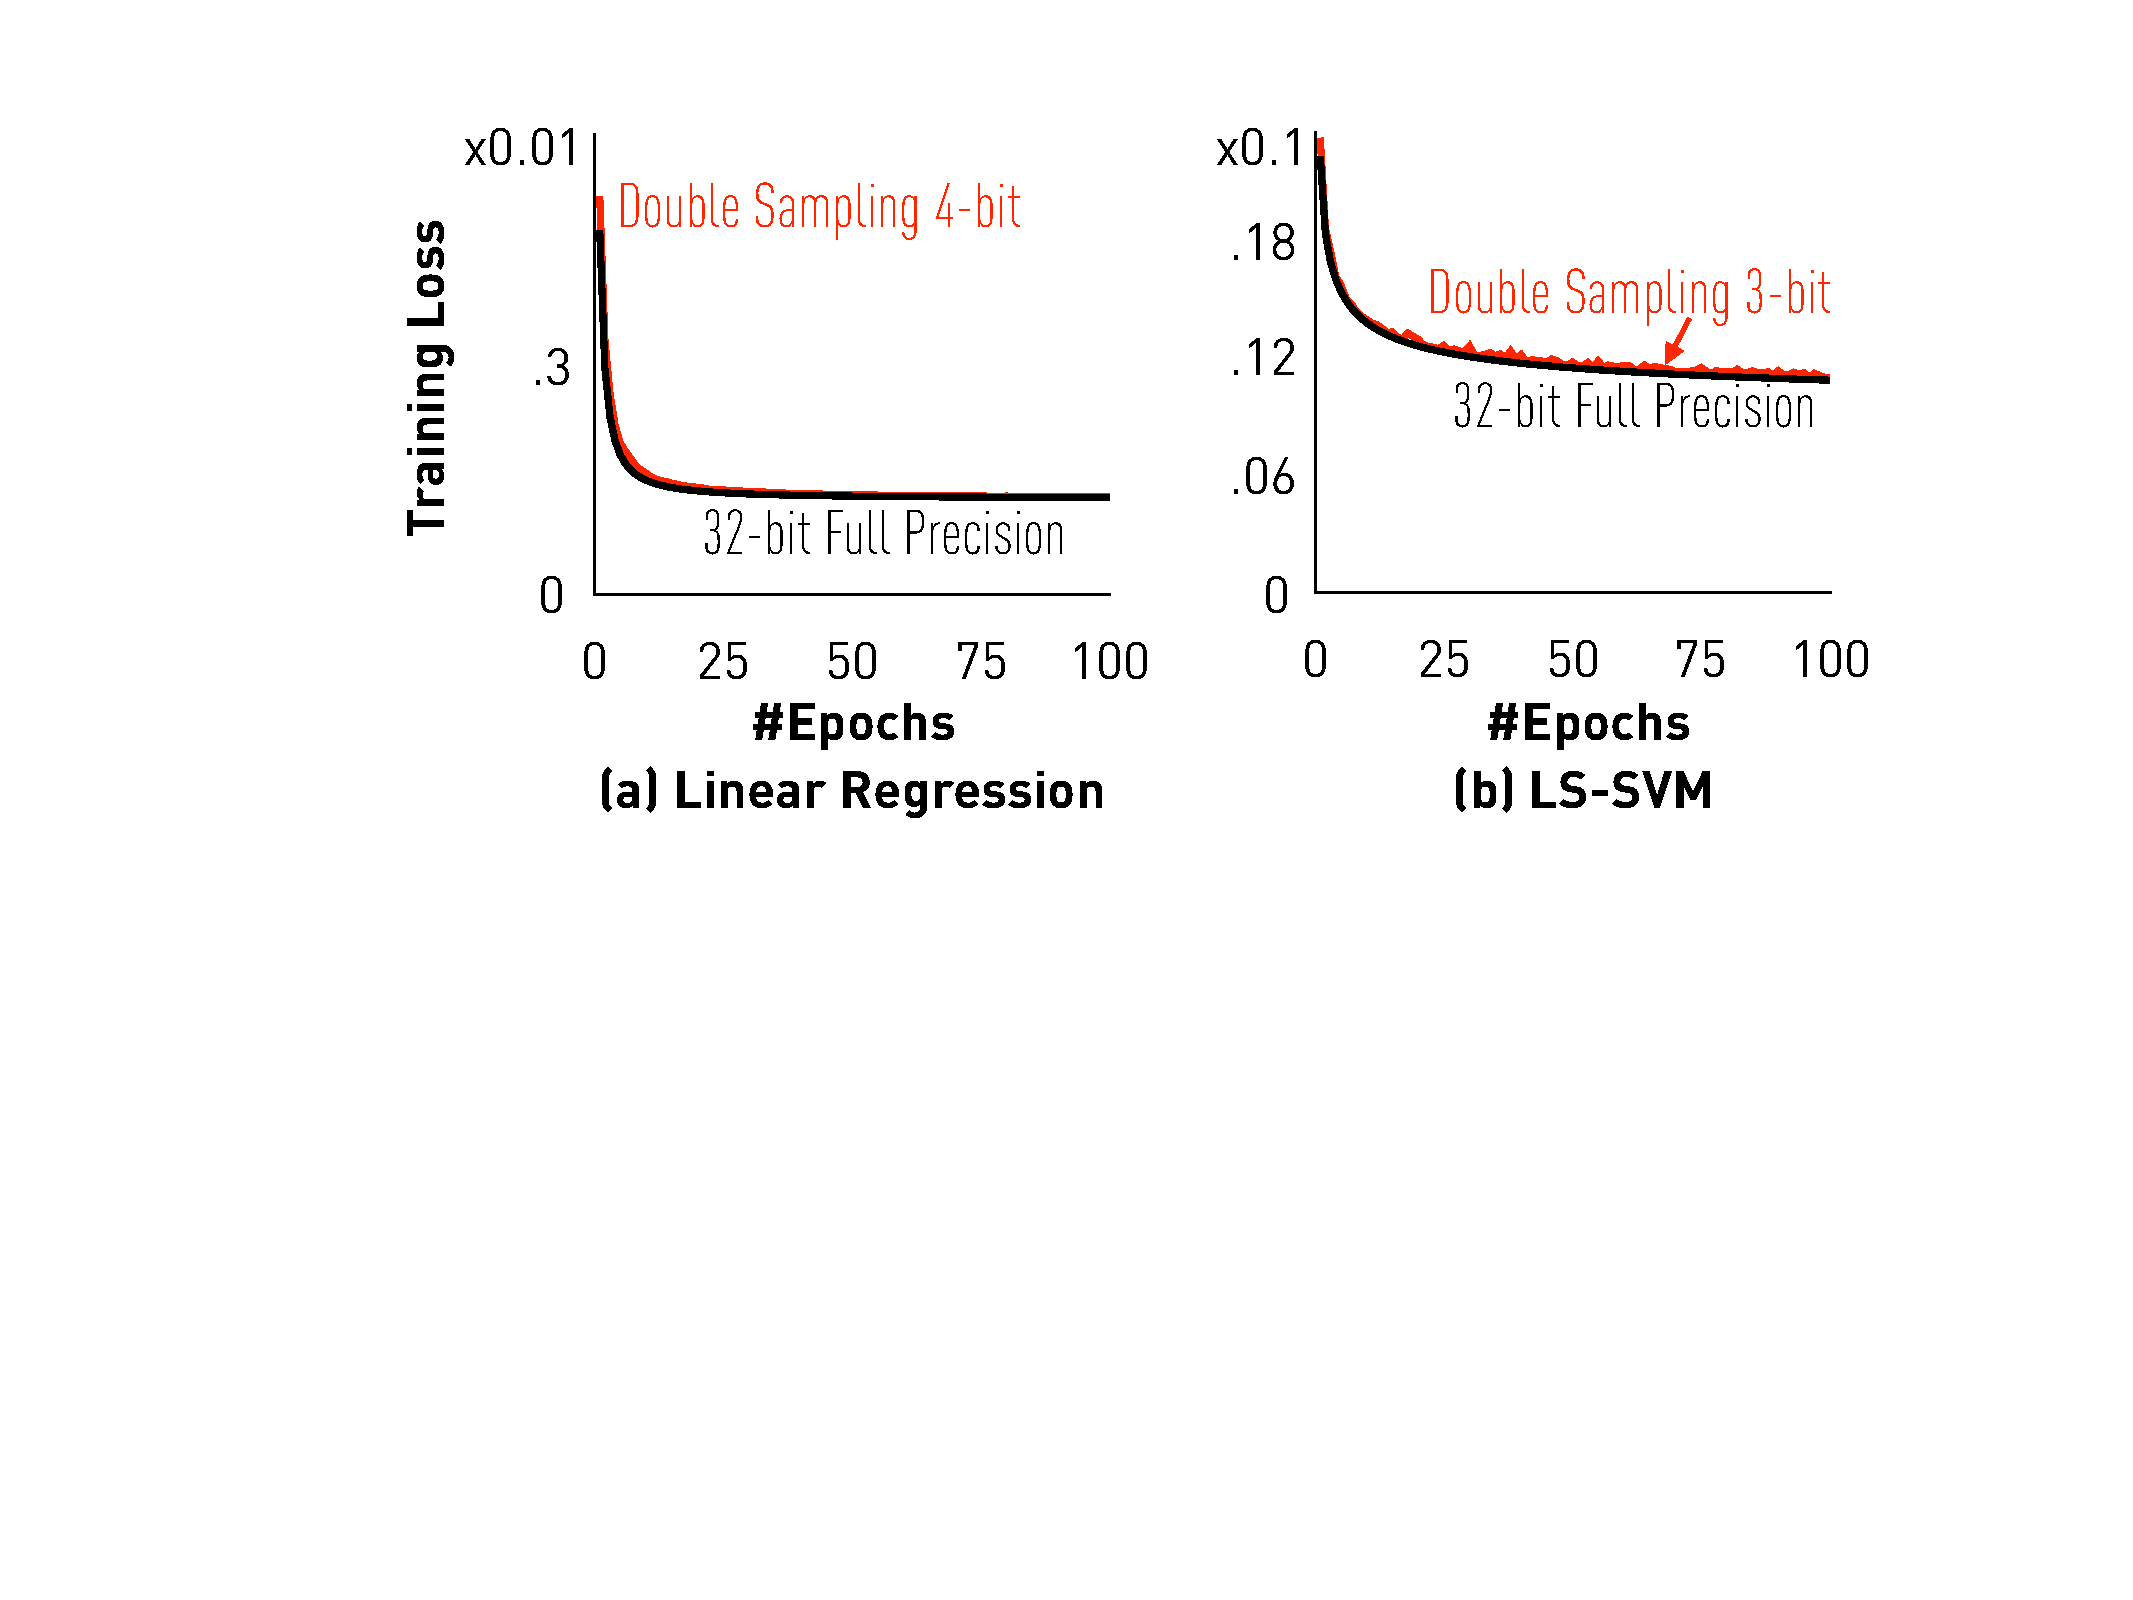
\includegraphics[width=0.7\columnwidth]{final-experiments/linearmodel} 
\vspace{-1em}
\caption{Linear models with end-to-end low precision.}
\label{fig:convergence}
\end{figure}

\vspace{-1em}
\subsection{Linear Models}
\vspace{-0.5em}

For linear models, we validate that (1) 
with double sampling, SGD with low
precision converges---in
comparable empirical 
convergence rates---to the same solution
as SGD with full precision; and
(2) implemented on FPGA, our low-precision
prototype achieves significant speed-up
because of the decrease of bandwidth
consumption.

\vspace{-1em}
\paragraph{Convergence}

Figure~\ref{fig:convergence} illustrates
the result of training linear models:
(a) linear
regression and (b) least squares SVMs,
with end-to-end low-precision and 
full precision. For
low precision, we pick the 
smallest number of bits that
result in a smooth convergence
curve. We compare the final 
training loss in both settings 
and the convergence rate.

We see that, for both linear regression 
and least squares SVM,
using 3 or 4-bit is always enough
to converge to the same solution
with comparable convergence rate. 
This validates our prediction that
double-sampling provides an
unbiased estimators of the gradient.
Considering the size of input
samples that we need to read, we
could potentially save 8-10$\times$ 
memory bandwidth compared to using 
32-bit. 

\vspace{-1em}
\paragraph{Speedup}
We implemented our low-precision 
framework on a state-of-the-art 
FPGA platform. We leave the detailed 
implementation and the circuit to
the full version of this paper. 
This implementation assumes the input
data is already quantized and
stored in memory (quantized
data can be generated during the
first epoch of training.)

Figure~\ref{fig:speedup} illustrates 
the result of (1) our FPGA
implementation with quantized data,
(2) FPGA implementation with 32-bit
data, and (3) Hogwild! running with
10 CPU cores.
Observe that all approaches
converge to the same solution.
FPGA with quantized data converges
6-7$\times$ faster
than FPGA with full precision
or Hogwild!. The FPGA implementation
with full precision is
memory-bandwidth bound, and by using our framework on quantized data, we save 
up to 8$\times$ memory-bandwidth, which
explains the speedup.


\begin{figure}[t]
\centering
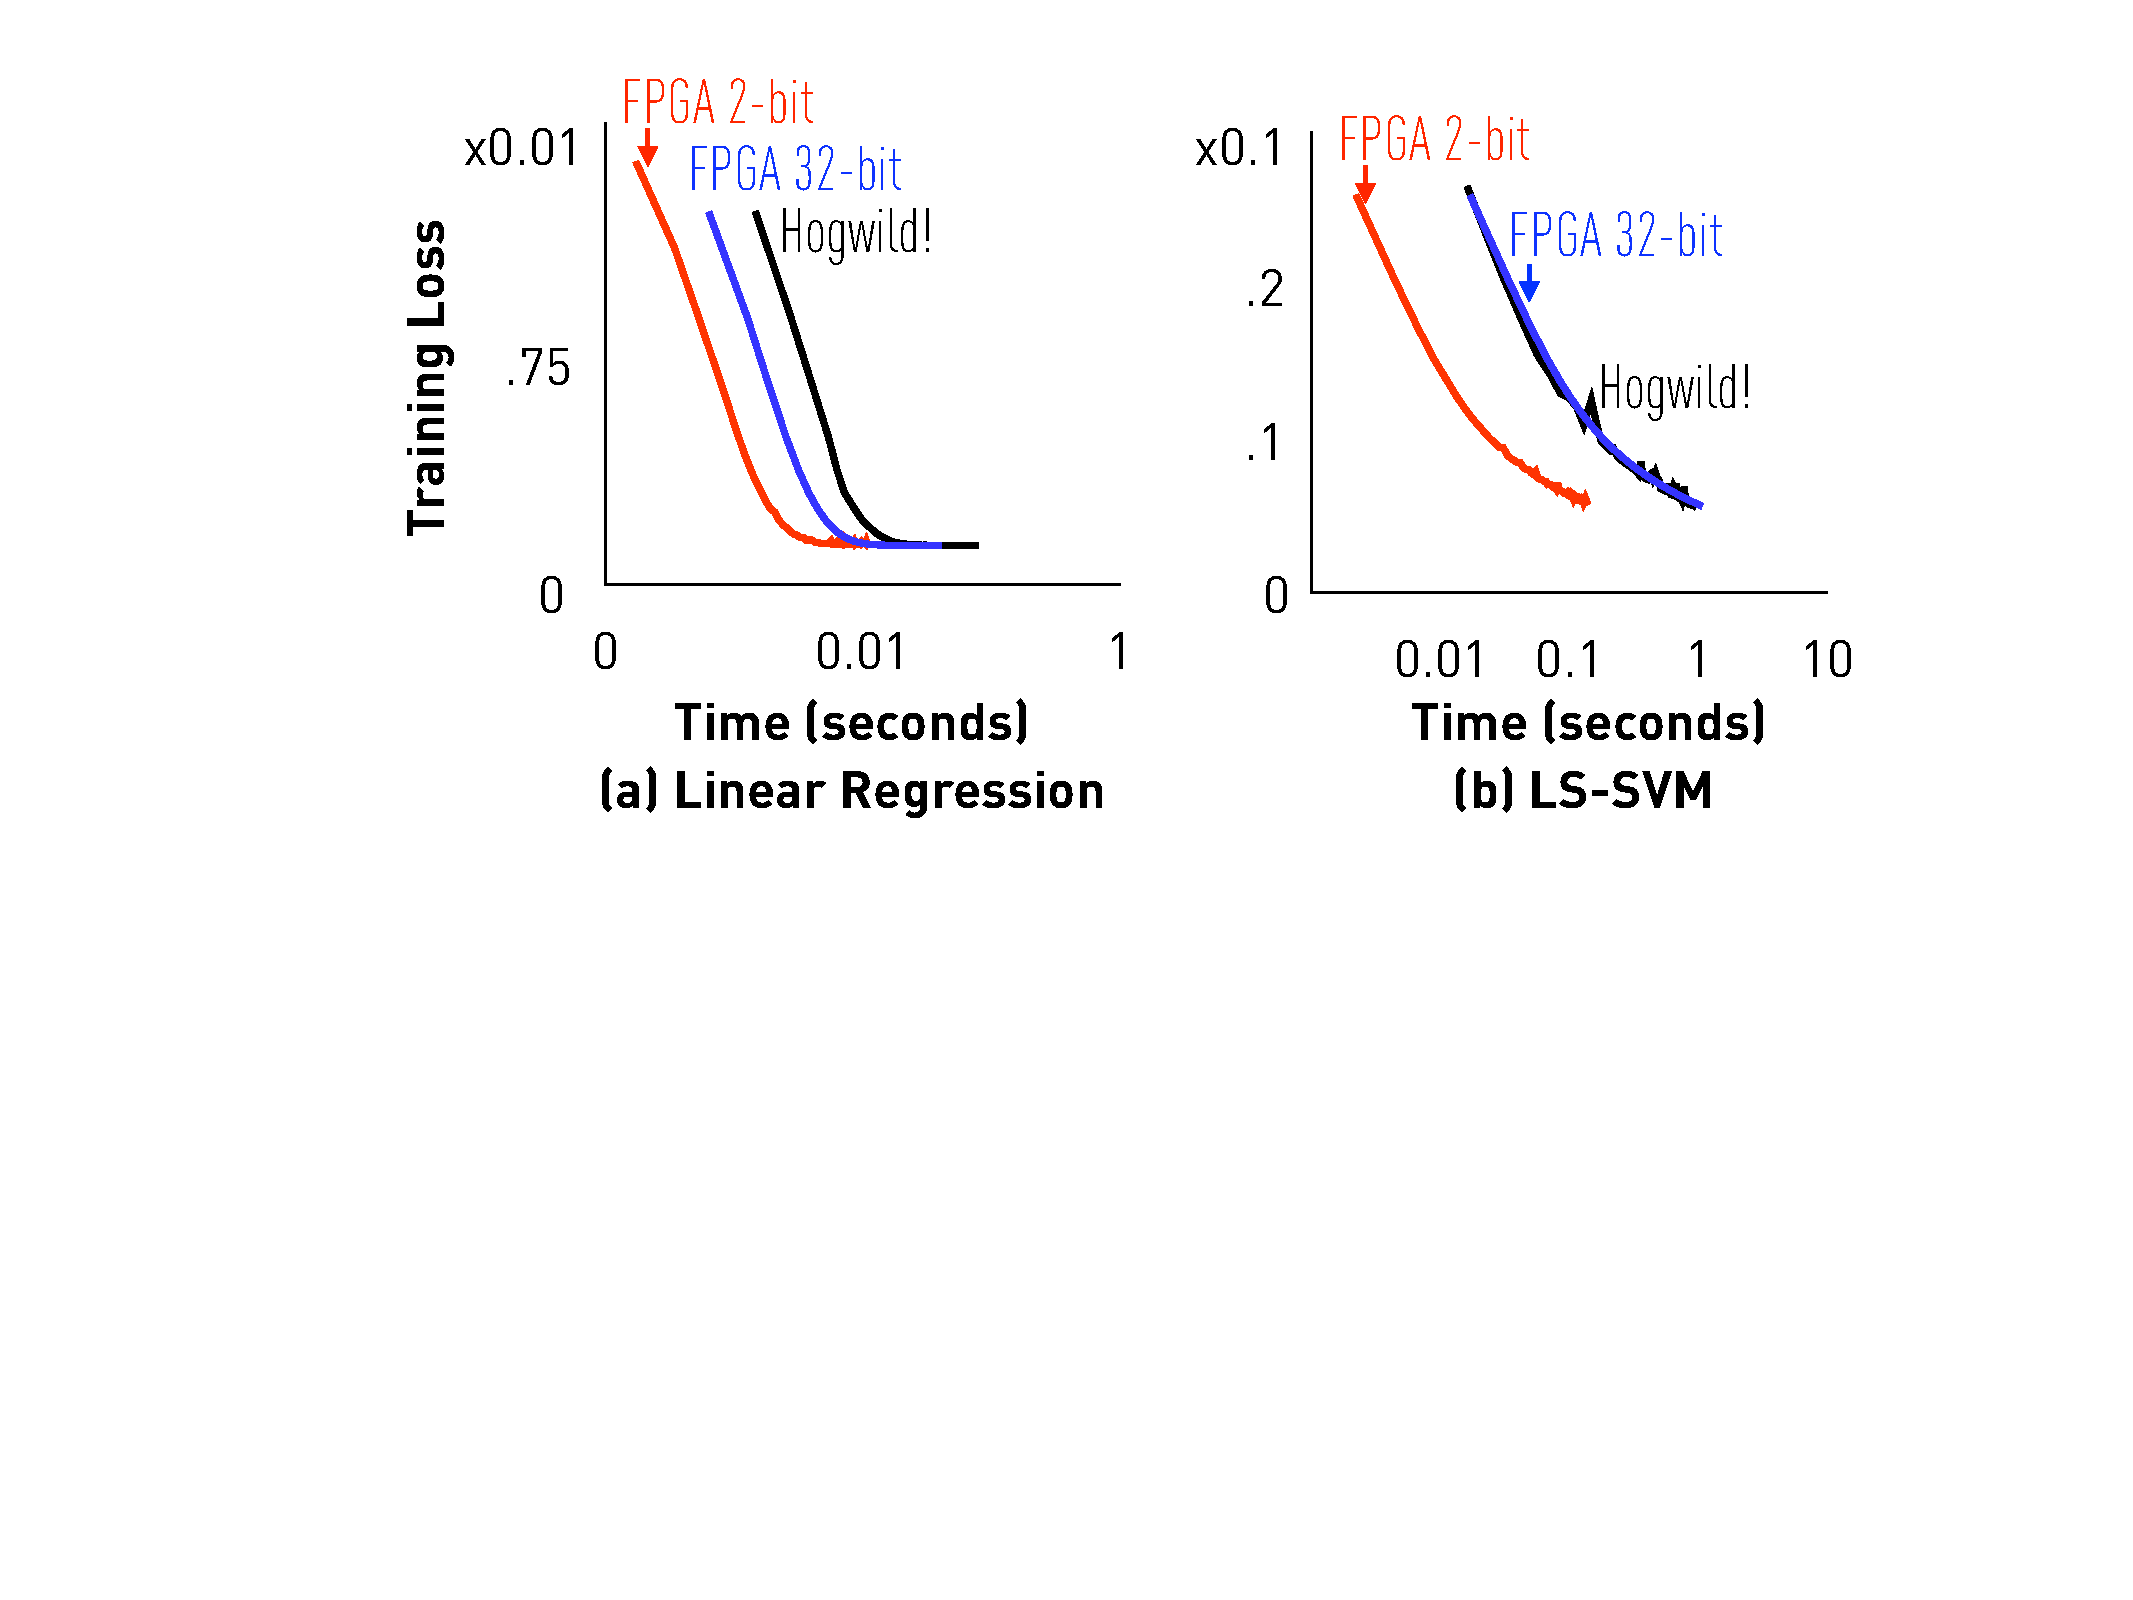
\includegraphics[width=0.7\columnwidth]{final-experiments/linear-fpga} 
\vspace{-1em}
\caption{FPGA implementation of linear models.}
\label{fig:speedup}
\end{figure}

\vspace{-1em}
\subsection{Non-Linear Models}
\vspace{-0.5em}

We validate that (1) our Chebyshev 
approximation approach is able to
converge to almost the same solution 
with 8-bit precision for both SVM
and logistic regression;
and (2) however, we are able to construct
a strawman with 8-bit deterministic 
rounding or naive stochastic rounding
to achieve the same quality and convergence 
rate.

\vspace{-0.5em}
\paragraph{Chebyshev Approximations}

Figure~\ref{fig:chebyshev} illustrates
the result of training SVM
and logistic regression 
with Chebyshev approximation. Here,
we use Chebyshev polynomials up to
degree 15 (which requires 16 samples
that can be encoded with 4 extra 
bits). For each sample, the precision
is 4-bit, and therefore, in total
we use 8-bit for each single number
in input samples. We see that 
with our quantization framework,
SGD converges to similar training loss 
with comparable empirical convergence 
rate for both SVM and logistic regression.
We also get no loss in test accuracy.

\begin{figure}[t]
\centering
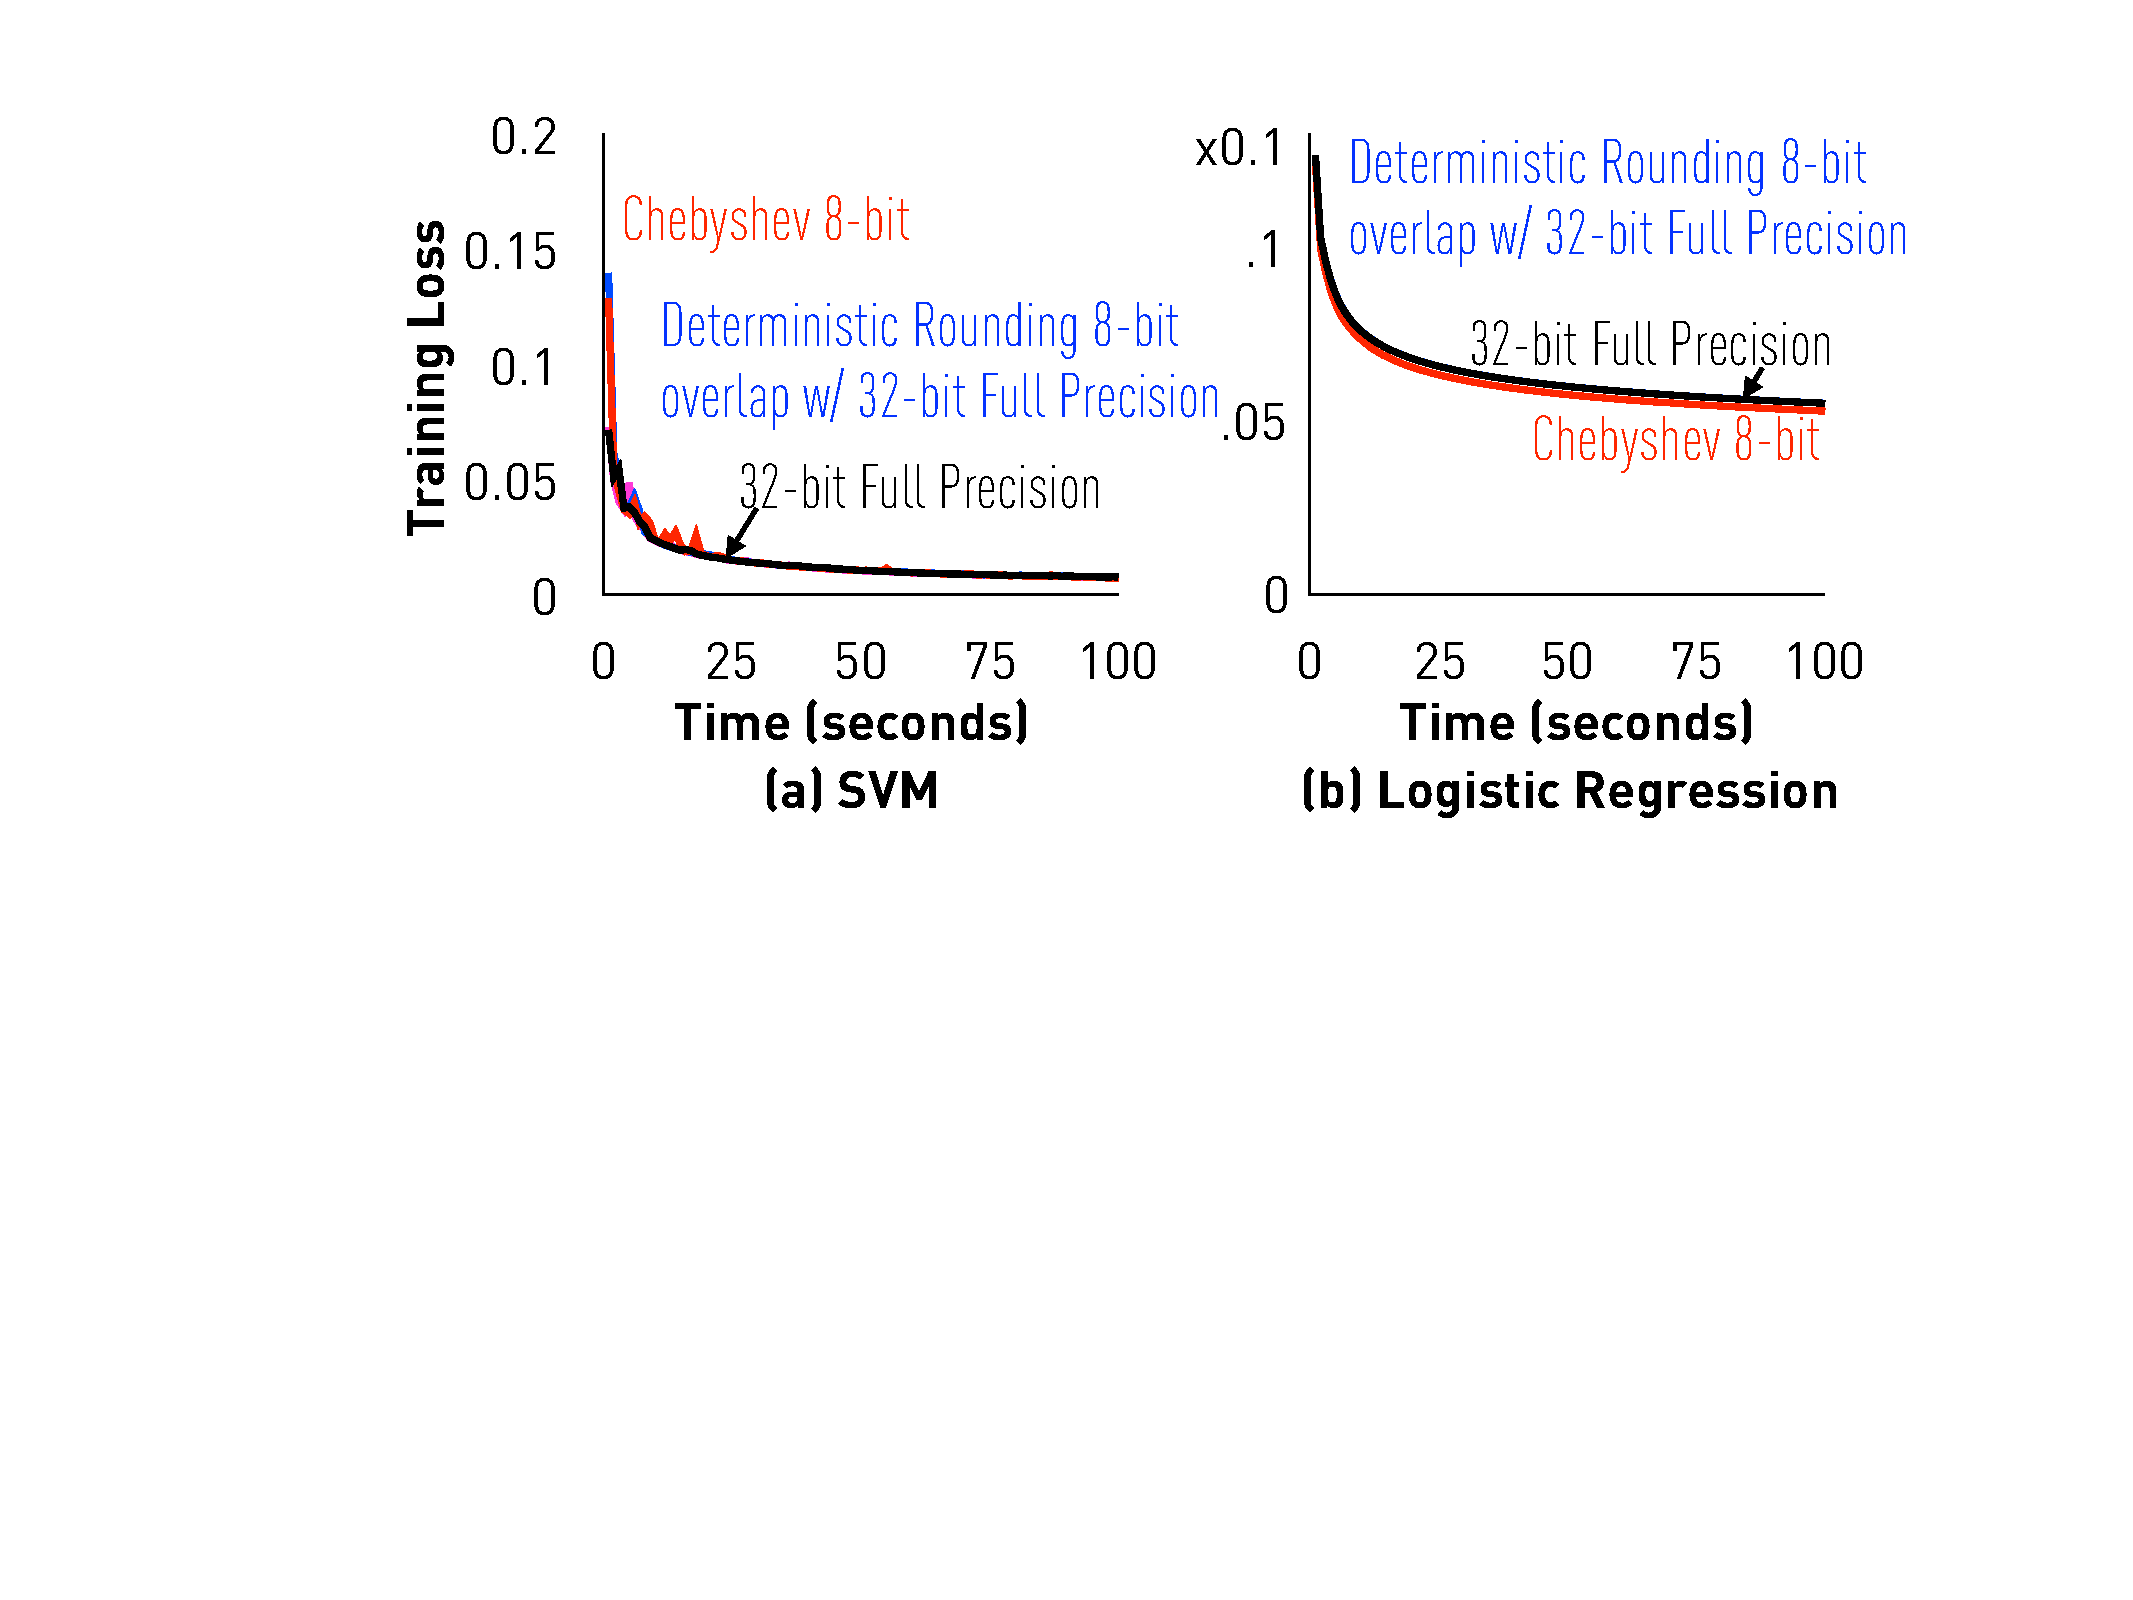
\includegraphics[width=0.7\columnwidth]{final-experiments/chebyshev} 
\vspace{-1em}
\caption{Non-linear models with Chebyshev approximation.}
\label{fig:chebyshev}
\end{figure}

\vspace{-0.5em}
\paragraph{Negative Results}

We are able to construct the following,
much simpler strategy that also
uses 8-bit to achieve the same quality
and convergence rate as our
Chebyshev. In practice, as both
strategies incur bias on the result,
we do {\em not} see strong reasons to
use our Chebyshev approximation, thus
we view this as a negative result.
As shown in Figure~\ref{fig:chebyshev},
if we simply round the input samples
to the nearest 8-bit fix point
representation (or do rounding
stochastically), we achieve the
same, and sometimes better,
convergence than our Chebyshev 
approximation.

\begin{figure}[t]
\centering
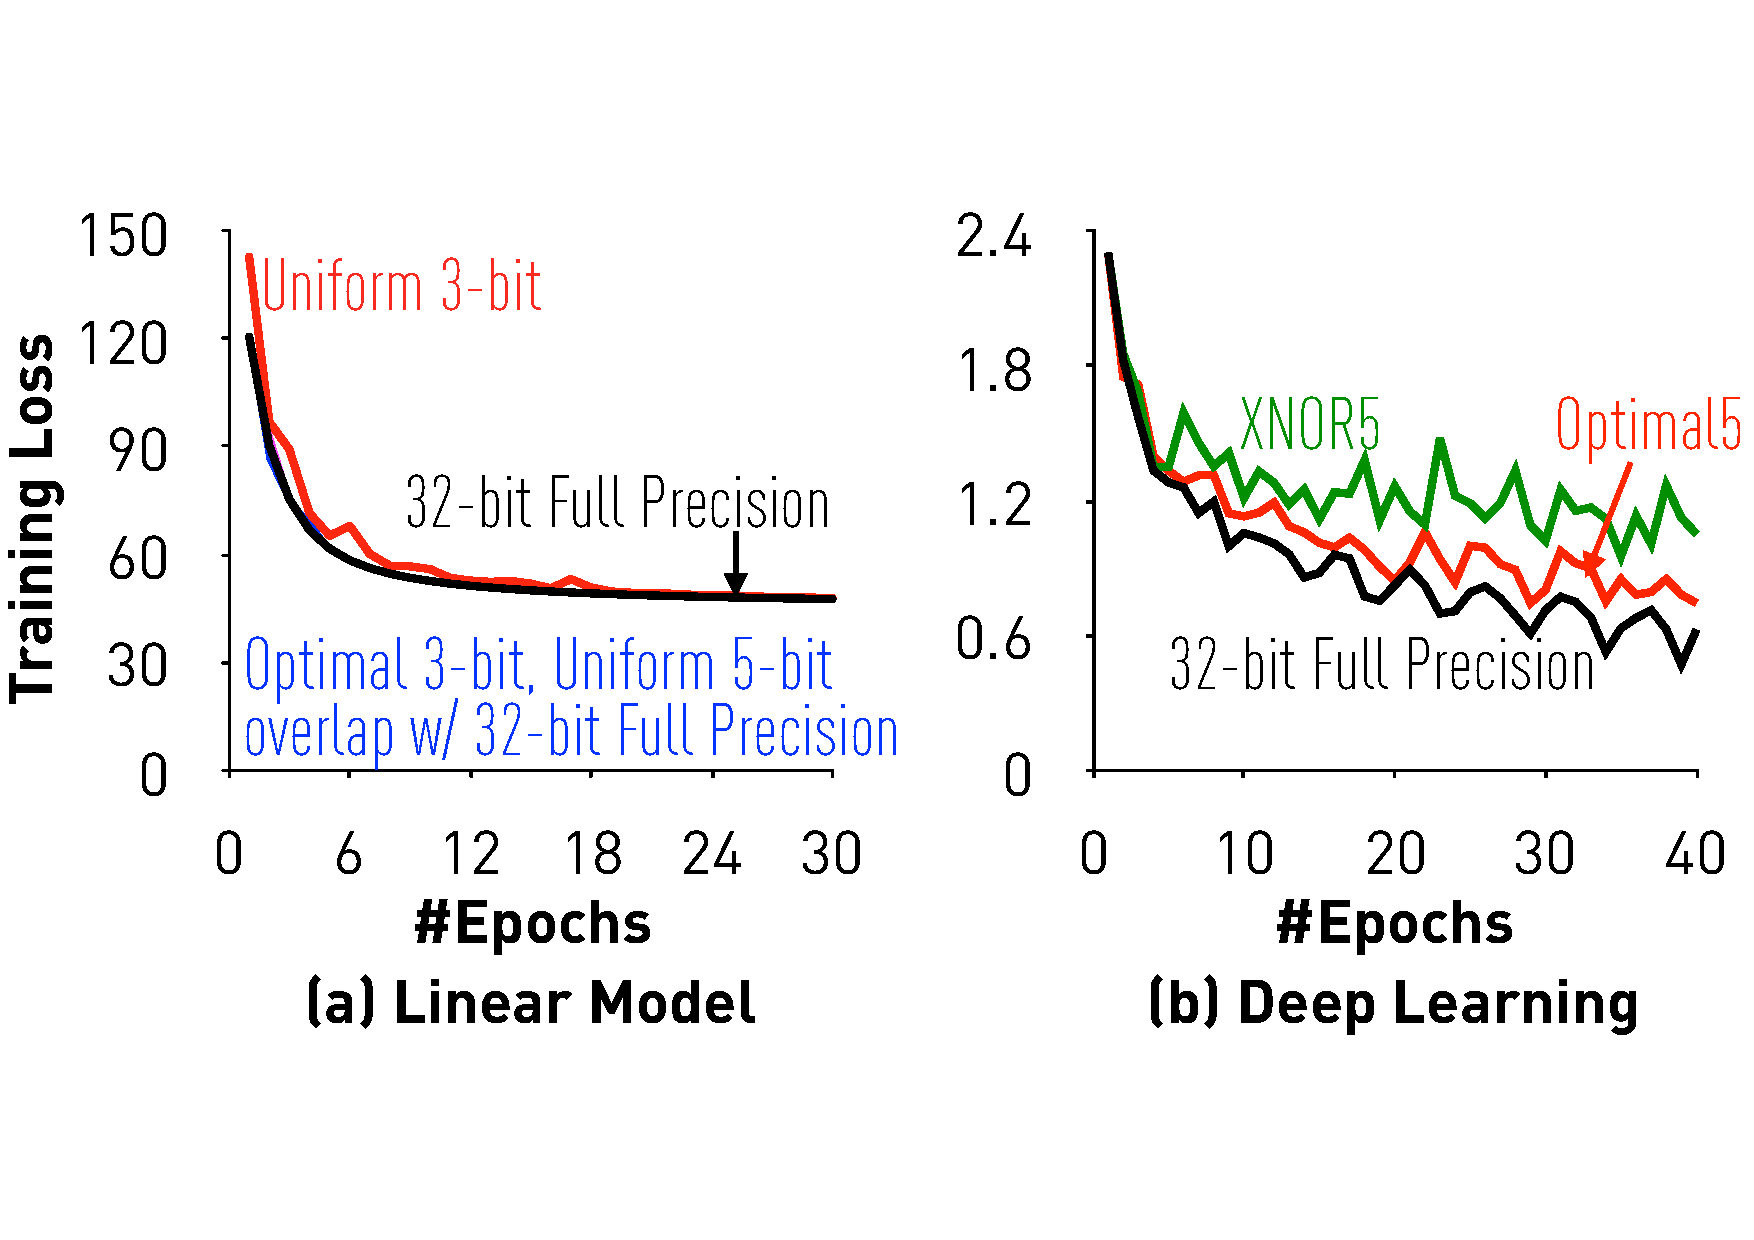
\includegraphics[width=0.7\columnwidth]{final-experiments/optimal} 
\vspace{-1em}
\caption{Optimal quantization strategy.}
\label{fig:optimal}
\end{figure}

\vspace{-0.5em}
\subsection{Data-Optimal Quantization Strategy}
\vspace{-0.5em}

We validate that, with our data-optimal quantization strategy, we can 
significantly decrease the number of 
bits that double-sampling requires to 
achieve the same convergence.
Figure~\ref{fig:optimal}(a) illustrates
the result of using 3-bit and 5-bit
for uniform quantization and optimal 
quantization on the {\bf YearPrediction}
dataset. We see that,
while uniform quantization needs 5-bit
to converge smoothly, optimal
quantization only needs 3-bit. 
We save almost $2\times$ number of 
bits by just allocating quantization points wisely.

\vspace{-0.5em}
\subsection{Extensions to Deep Learning}
\vspace{-0.5em}

We validate that our data-optimal quantization
strategy can be used in training deep neural
networks. We take Caffe's CIFAR-10 tutorial
and compare three different quantization
strategies: (1) Full Precision, (2) XNOR5, 
a XNOR-Net implementation that, follows
the multi-bits strategy in
the original paper, quantizes data into
five uniformly chosen levels, and (3)
Optimal5, our quantization strategy with
five optimal quantization levels. As
shown in Figure~\ref{fig:optimal}(b), Optimal5
converges to a significantly lower training 
loss compared with XNOR5. In terms of
testing accuracy, Optimal5 achieves a
near 10 points improvement over XNOR5.
This illustrates the improvement
one can get by training neural network with
a carefully chosen quantization strategy.


\vspace{-1em}
\section{Related Work} 

\vspace{-0.5em}
There are work on ``low precision SGD''~\cite{DeSa:NIPS:2015,Alistarh:2016:ArXiv}. 
Most of them provide
theoretical guarantee when the gradients are quantized.
The model and input samples, on the other hand, are much more difficult
to analyze because of the non-linearity. In this paper, 
we
focus on the {\em end-to-end}
quantization for all components.

\vspace{-1em}
\paragraph{Low-Precision Deep learning.}

Low-precision training of deep neural networks has been studied
intensively and many heuristics work well for a subset of networks.
OneBit SGD~\cite{Frank:2014:Interspeech} provides
a gradient compression heuristic developed in the context of deep 
neural networks for speech recognition. There are successful 
application of end-to-end quantization to training neural networks
resulting in little to no quality loss~\cite{hubara2016quantized,
rastegari2016xnor,zhou2016dorefa,miyashita2016convolutional,li2016ternary,gupta2015deep}. These work quantize weights, activations, and gradients 
to low-precision (e.g., 1-bit) and revise the backpropagation 
algorithm to be aware of the quantization function.
The empirical success of these work inspired this paper, in which we try
to provide a {\em theoretical} understanding of end-to-end low-precision
training for machine learning models.
Another line of research concerns about inference and model
compression of a pre-trained model~\cite{vanhoucke2011improving,gong2014compressing,Han:2016:ICLR,lin2016fixed,kim2016bitwise,kim2015compression,wu2016quantized}.
In this paper, we focus on training and leave the study of
inference as future work.

\vspace{-1em}
\paragraph{Low-Precision Linear Models.}

Quantization is a fundamental topic studied by the
DSP community, and there have been research related to
linear regression models in the presence of quantization
error or other type of noises. For example,
\citet{Gopi:2013:ICML} studied compressive sensing
with \textcolor{red}{binary} quantized measurement, and \textcolor{red}{a two stage algorithm was proposed to recover the sparse high precision solution up to a scale factor.}
%algorithm focuses on getting a high-precision solution with low-precision computation. 
Also, the
classic errors-in-variable model~\cite{Hall:2008:Book}
could also be relevant if quantization is treated 
as a source of ``error''. In this paper, we scope
ourselves to the context of stochastic gradient descent, 
and our insights go beyond simple linear models.

\vspace{-1em}
\paragraph{Other Related Work.} Precision of data
representation is a key design decision
for configurable hardwares such as FPGA. There are attempts to
lower the precision when training machine learning models
on these hardware~\cite{Kim:2011:ICASSP}. 
These results are mostly empirical; we
aim at providing a theoretical understanding, which 
enables new algorithms that are not covered 
by these references.

\vspace{-1em}
\section{Discussion and Future Work}
\label{sec:conclusions}

The motivating question of this paper was whether end-to-end low-precision data representation can enable efficient computation, while maintaining convergence guarantees. 
We have shown that a relatively simple stochastic quantization framework can achieve this for linear models. 
Moreover, for this setting, as little as two bits per model dimension are sufficient for good accuracy, and can enable a high-performance FPGA implementation.  

For non-linear models, the picture we observe is more nuanced. 
In particular, we find that our framework can be generalized to this setting, and that in practice \emph{8 bit precision is sufficient} to achieve good accuracy on a variety of tasks, such as SVM and logistic regression. 
However, in this setting, naive rounding has similar performance. 

It is interesting to consider the rationale behind these results. On one hand, our framework is based on the idea of \emph{unbiased approximation} of the original SGD process. For linear models, this is easy to achieve. For non-linear models, this is harder, and we must focus on guaranteeing arbitrarily low bias. 
However, for a variety of interesting functions, such as hinge loss, guaranteeing low bias requires high polynomial approximations. In turn, these increase the variance (since variance bounds are exponential in the degree). These two constraints force us to increase the \emph{density} of the quantization, in order to achieve good approximation guarantees. 

In future work, we plan to examine compressed data representations which are not necessarily (approximate) unbiased estimators of the high-precision process. 
Such representations, for instance based on naive rounding with feedback error correction~\cite{1BitSGD}, have been successfully employed for gradient compression, although they currently are not known not provide any guarantees. Since the resulting processes no longer approximate standard SGD, the analysis appears non-trivial. 

An independent contribution of our work is a set of algorithms for finding an optimal quantization with respect to variance. 
We show that improved quantizations can significantly improve accuracy for training in both convex and non-convex settings. 
In future work, we plan to explore the potential of these techniques for training and inference.  

\cleardoublepage





\bibliographystyle{icml2017}
\bibliography{low-precision.bib}


\end{document}
